\documentclass[letter, 10pts]{article}
\usepackage[monocolor]{../math232/ahsansabit}
\usepackage[]{float}
\usepackage{tikz}
\usepackage{tikz-3dplot}
\usepackage[outline]{contour} % glow around text
\usepackage{xcolor}
\usepackage{pdfpages}
\usepackage{physics}
\usepackage[]{hyperref}
\usepackage{multicol}
\title{Classical Mechanics : : Homework 10}
\author{Ahmed Saad Sabit, Rice University}
\date{\today}
\newcommand{\hb}{\hbar}
\newcommand{\U}{\uparrow}
\newcommand{\D}{\downarrow}
\usepackage[]{braket}
\begin{document}
\maketitle

\section*{Problem 01} 
\hrule
The equations of torque are 
\begin{align*}
	\tau_1 &= I_1 \dot{\omega}_1 + (I_3 - I_2) \omega_3 \omega_2 \\ 
	\tau_2 &= I_2 \dot \omega_2 + (I_1 - I_3) \omega_1 \omega_3 \\ 
	\tau_3 &= I_3 \dot \omega_3 + (I_2 - I_1) \omega_2 \omega_1 
\end{align*}
Without losing generality let us assume $I_1 < I_2 < I_3$. So Dzhanibekov Effect, or Tennis Racket Theorem, says that $I_2$ moment of inertia is the one that is along the unstable principle axis.

\subsection*{Unstability along $I_2$ }
Let's look at an initial $\Omega$ rotating only along $(0,1,0)$ (the unstable axis). Note that we are working in the basis where the unit vectors are the principle axis. 

Let's have a slight perturbation along for angular velocity $(1,0,0)$ that is $\delta$ which says 
\[
	(0, \Omega, 0) \to (\delta, \Omega, 0)
\] 
The external torques are zero. Then using the above perturbation to find the rate of change of $\omega$ for the initial moment
\begin{align*}
	\tau_1 &=  0 \implies \dot{\omega}_1 = 0 \\ 
	\tau_2 &=  0 \implies \dot \omega_2 = 0 \\ 
	\tau_3 =0 &= I_3 \dot \omega_3 + (I_2 - I_1) \Omega \delta  \implies \dot \omega_3 = - \frac{I_2 - I_1}{I_3} \Omega \delta
\end{align*}
Hence after some infinitesimal time $\Delta t$ we get $\omega_3$ to be 
\[
	\omega_3 \approx - \frac{I_2 - I_1}{I_3} \Omega \delta \Delta t
\] 
Now, with the new $\omega_3$ iteration, the Euler's equations are (external torque is still 0)
\begin{align*}
\dot{\omega}_1 &= - \frac{I_3 - I_2}{I_1} \left(- \frac{I_2 - I_1}{I_3} \Omega \delta \Delta t\right) \Omega 
=
\frac{(I_3 - I_2)(I_2 - I_1)}{I_1 I_3} \Omega^2 \delta \Delta t > 0
\\
\dot \omega_2 &= - \frac{I_1 - I_3}{I_2} \delta \left(- \frac{I_2 - I_1}{I_3} \Omega \delta \Delta t\right) = - 
\frac{(I_3 - I_1)(I_2 - I_1)}{I_3 I_2} \Omega \delta^2 \Delta t\\
\end{align*}
Being a little bit more sloppy with the mathematics we take a derivative

\begin{align*}
\ddot{\omega}_1 &=
\frac{(I_3 - I_2)(I_2 - I_1)}{I_1 I_3} \Omega^2 \delta 
\\
\ddot \omega_2 
		&= - 
\frac{(I_3 - I_1)(I_2 - I_1)}{I_3 I_2} \Omega \delta^2  \\
\end{align*}
We can see above that $\omega_1$'s second derivative grows rapidly for a small perturbation $\delta$. This is an exponentially growing motion, instead of an oscillatory one. So the overall direction of rotation does not stay long $\left( 0 , \Omega , 0 \right) $ for the whole motion, implying $(0,1,0)$ direction of rotation to be unstable. 

We picked this to be the direction of $I_2$ when $I_1 < I_2 < I_3$. So this principal axis is unstable. 

This exact same calculation for $(0, \Omega, \delta)$ perturbation will give the exact same exponential growth along perturbation. 

\subsection*{Stability along $I_1$ (or $I_3$)}
Let's start from $\vec{\omega} = \left(\Omega, 0,0\right)$ and then introduce a general perturbation $\left(\Omega, \epsilon_2, \epsilon_3\right)$

\begin{align*}
0 &= \dot{\omega}_1 + \frac{I_3 - I_2}{I_1} \epsilon_2 \epsilon_3 \\
0 &= \dot \epsilon_2 + \frac{I_1 - I_3}{I_2} \Omega \epsilon_3 \\
0 &=  \dot \epsilon_3 + \frac{I_2 - I_1}{I_3} \Omega \epsilon_2
\end{align*}
Fix the signs if necessary 
\begin{align*}
0 &= \dot{\omega}_1 + \frac{I_3 - I_2}{I_1} \epsilon_2 \epsilon_3 \\
0 &= \dot \epsilon_2 - \frac{I_3 - I_1}{I_2} \Omega \epsilon_3 \\
0 &=  \dot \epsilon_3 + \frac{I_2 - I_1}{I_3} \Omega \epsilon_2 \\
  &\implies \text{Contract the notations} \\  
0 &= \dot{\omega}_1 + A \epsilon_2 \epsilon_3 \\
0 &= \dot \epsilon_2 - B \Omega \epsilon_3 \\
0 &=  \dot \epsilon_3 + C \Omega \epsilon_2 \\
\end{align*}
Let's look at the perturbation's differential equations 
\begin{align*}
0 &= \dot \epsilon_2 - B \Omega \epsilon_3 \\
0 &=  \dot \epsilon_3 + C \Omega \epsilon_2 \\
  & \implies \text{Take on derivative}  \\ 
0 &= \ddot \epsilon_2 - B \Omega \dot \epsilon_3  = \ddot \epsilon_2 + BC \Omega \epsilon_2 = 0\\
0 &=  \ddot \epsilon_3 + C \Omega \dot \epsilon_2 = \ddot{\epsilon}_3 + BC \Omega \epsilon_3 = 0\\
\end{align*}
We get simple harmonic equations for the perturbations. So they don't make any noticeable difference other than just small precession like motion. 

Given the amplitude of the perturbation being small, we can simply see that $\dot{\omega}_1 \approx 0$. For this we can say that $I_1$ is a stable principle axis direction. 

Because of the symmetry of the equations, just flipping the notations will immediately prove the exact same reasoning for $I_3$ too. So we proved that Mr. Dzanibekov was right (or Tennis Racket Theorem is true). 


Veritasium in youtube has made a nice video on this matter. 





\newpage
\section*{Problem 02} 
\hrule 

\subsection*{(a)} 
For the hollow sphere, the inertia tensor is not going to have any off diagonal elements because of the symmetry (symmetry being any principle axis has the same moment of inertia given the origin is in the center of the ball). Also it's going to be a multiple of the Identity Matrix because of the spherical symmetry. 

Through any axis crossing the center, the moment of inertia can be easily computed. 

\[
I_{ij} = \int_V \rho \left( r^2 \delta_{ij} - x_i x_j \right) \, dV
\]
For our case $I_{11}, I_{22}, I_{33}$ are the same thing. And any off diagonals are zero. 
\[
\rho = \frac{M}{\frac{4}{3} \pi (a^3 - b^3)}
\]

\[
I = \int_V \rho r^2 \sin^2\theta \, dV
\]
For the sphere
\[
dV = r^2 \sin\theta \, dr \, d\theta \, d\phi
\]
Take the integral 
\[
I = \rho \int_b^a \int_0^\pi \int_0^{2\pi} r^4 \sin^3\theta \, d\phi \, d\theta \, dr
\]
$\phi$ symmetry
\[
\int_0^{2\pi} 1 \, d\phi = 2\pi
\]
Latitude integral 
\[
\int_0^\pi \sin^3\theta \, d\theta = \int_0^\pi (1 - \cos^2\theta) \sin\theta \, d\theta = \left[ -\frac{\cos\theta}{3} + \frac{\cos^3\theta}{3} \right]_0^\pi = \frac{4}{3}
\]
Radius from $b$ to $a$ 
\[
\int_b^a r^4 \, dr = \frac{1}{5} \left[ r^5 \right]_b^a = \frac{1}{5} (a^5 - b^5)
\]
Put everything together 
\[
I = \rho \cdot 2\pi \cdot \frac{4}{3} \cdot \frac{1}{5} (a^5 - b^5) = \frac{8\pi}{15} \rho (a^5 - b^5)
\]

\[
I = \frac{8\pi}{15} \cdot \frac{M}{\frac{4}{3} \pi (a^3 - b^3)} \cdot (a^5 - b^5)
\]

\[
I = \frac{2M}{5} \cdot \frac{a^5 - b^5}{a^3 - b^3}
\]

So the tensor is 
\[
\hat{I} = 
\frac{2M}{5} \cdot \frac{a^5 - b^5}{a^3 - b^3}
\begin{bmatrix} 1 & 0 & 0 \\ 0 & 1 & 0 \\ 0 & 0 & 1 \end{bmatrix} 
\] 





\subsection*{(b)} 
Angular impulse applied by cue ($r$ distance from center)
\[
\tau \Delta t = r F \Delta t = r \Delta p    
\] 
Angular impulse received by ball
\[
\Delta L = L - 0 = I \omega  
\] 
They should be equal 
\begin{equation}
r \Delta p = I \omega
\end{equation}
Linear momentum gained is $\Delta p$. Invoke no slip condition then 
\[
\omega = \frac{v}{a} = \frac{\Delta p}{m a}
\] 
Use this with (1) then 
\[
r \Delta p = I \frac{\Delta p}{m a} \implies r = \frac{I}{ma}
\] 
What we get for $H$ is 
\[
H = r + a = \frac{I}{ma} + a
\] 
In this case it will be 
\[
H = \frac{2}{5 a} \frac{a^{5} - b^{5}}{a^{3} - b^{3}} + a  
\] 



\subsection*{(c)} 
\subsubsection*{$b = 0$ Solid Sphere} 
\begin{align*}
H = \frac{2}{5 a} a^2 + a = \frac{2}{5} a + a = \frac{7}{5} a   
\end{align*}

\subsubsection*{$b \to  a$ Thin Sphere} 
\begin{align*}
	H &= \frac{2}{5 a} \frac{a^{5} - b^{5}}{a^{3} - b^{3}} + a \\  
	  &=
	\frac{2}{5 a} \frac{a^{5} - (a - \varepsilon)^{5}}{a^{3} - (a - \varepsilon)^{3}} + a   \\
	  &=
	\frac{2}{5 a} \frac{a^{5} - a^{5}(1 - \frac{\varepsilon}{a})^{5}}{a^{3} - a^{3}(1 - \frac{\varepsilon}{a})^{3}} + a   \\
	  &\approx 
	\frac{2}{5 a} \frac{a^{5} - a^{5}(1 -5\frac{\varepsilon}{a})}{a^{3} - a^{3}(1 - 3\frac{\varepsilon}{a})} + a   \\
	  &= 
	\frac{2}{5 a} \frac{a^{5} ( 1 - 1 +5\frac{\varepsilon}{a})}{a^{3} (1 - 1 + 3\frac{\varepsilon}{a})} + a   \\
	  &= 
  \frac{2}{3 a} {a^{2}} + a 
 \\ 
& = 
\frac{2}{3} a + a = \frac{5}{3} a  
\end{align*}







\newpage
\section*{Problem 03}
\hrule 


Call $I_1 = I_2 = I_x = I_y$. Then
\[
\vec{\omega} = (\omega_1 , 0 , \omega_3)
\] 
Let the angular velocity of the space station be \( \vec{\omega} = (\omega_1, 0, \omega_3) \) in the body frame before the torque is applied. The torque \( \vec{\Gamma} = (0, 0, \Gamma) \) acts along the \( z \)-axis, which is a principal axis. The Euler equations for a rigid body in the body frame are

\[
\begin{aligned}
I_1 \dot{\omega}_1 - (I_2 - I_3) \omega_2 \omega_3 &= 0 \\
I_2 \dot{\omega}_2 - (I_3 - I_1) \omega_3 \omega_1 &= 0 \\
I_3 \dot{\omega}_3 - (I_1 - I_2) \omega_1 \omega_2 &= \Gamma
\end{aligned}
\]

Initially when $\vec{\omega} = (\omega_1, 0, \omega_3)$ and $I_1 = I_2$
\[
\begin{aligned}
I_1 \dot{\omega}_1 &= 0 \\
I_2 \dot{\omega}_2 - (I_3 - I_1) \omega_3 \omega_1 &= 0 \\
I_3 \dot{\omega}_3  &= \Gamma
\end{aligned}
\]








Let's solve this problem for a general $\vec{\omega} = (\omega_1, \omega_2, \omega_3)$ and the initial condition will be invoked as $\vec{\omega_0} =( \omega^{0}_1, 0 , \omega^{0}_3 )$

\[
\begin{aligned}
\dot{\omega}_1 - \frac{I_2 - I_3}{I_1} \omega_2 \omega_3 &= 0 \\
 \dot{\omega}_2 - \frac{I_3 - I_1}{I_2} \omega_3 \omega_1 &= 0 \\
 \dot{\omega}_3 - \frac{I_1 - I_2}{I_3} \omega_1 \omega_2 &= \frac{\Gamma}{I_3}
\end{aligned}
\]

$I_1 = I_2 = I$ 
\[
\begin{aligned}
\dot{\omega}_1 - \frac{I - I_3}{I} \omega_2 \omega_3 &= 0 \\
 \dot{\omega}_2 - \frac{I_3 - I}{I} \omega_3 \omega_1 &= 0 \\
 \dot{\omega}_3  &= \frac{\Gamma}{I_3}
\end{aligned}
\]
Define
\[
 \frac{I - I_3}{I}  = \Lambda
\] 
Apply 
\[
\begin{aligned}
\dot{\omega}_1 - \Lambda \omega_2 \omega_3 &= 0 \\
 \dot{\omega}_2 + \Lambda  \omega_3 \omega_1 &= 0 \\
 \dot{\omega}_3  = \frac{\Gamma}{I_3} \implies \omega_3 &= \frac{\Gamma}{I_3} t + \omega^{0}_3
\end{aligned}
\]


\[
\begin{aligned}
\ddot{\omega}_1 - \Lambda  \omega_3 \dot \omega_2 &= 0
\implies \ddot{\omega}_1 - \Lambda \omega_3 (- \Lambda \omega_3 \omega_1) 
\implies \ddot{\omega}_1 + \Lambda^2 \omega_3^2 \omega_1 = 0
\\
 \ddot{\omega}_2 + \Lambda  \omega_3 \dot \omega_1 &= 0
 \implies \ddot{\omega}_2 + \Lambda \omega_3 \left(\Lambda \omega_2 \omega_3\right)
 \implies \ddot{\omega}_2 + \Lambda^2 \omega_3^2 \omega_2 = 0
\end{aligned}
\]


Equations of motion we are left with 
\begin{align*}
	\ddot{\omega}_1 + \Lambda^2 \omega_3^2 \omega_1 &= 0 \\ 
	\ddot{\omega}_2 + \Lambda^2 \omega_3^2 \omega_2 &= 0 \\ 
	\omega_3 &= \frac{\Gamma}{I_3}t + \omega_3^{0}
\end{align*}
\[
\boxed{
\vec{\omega} = 
\begin{bmatrix} 
	\omega_1^{0} \cos( \frac{I - I_3}{I}\left[ \frac{\Gamma}{I_3}t + \omega_3^{0}\right]t )
	\\
	\
	\\
	\omega_1^{0} \sin( \frac{I - I_3}{I}\left[ \frac{\Gamma}{I_3}t + \omega_3^{0}\right]t )
	\\ 
	\
	\\
	\frac{\Gamma}{I_3}t + \omega_3^{0}
\end{bmatrix} 
}
\] 
\textbf{Description of motion}
Rotation along axis of symmetry of the object increases because of the constant torque being provided. 

The precession frequency is given by function of time
\[
\Omega = \sqrt{\Lambda^2 \omega_3^2}  =  \frac{I-I_3}{I} \left(
\frac{\Gamma}{I_3}t + \omega_3^{0}\right)
\] 
The precession increases overtime and gets faster arbitrarily. 

































\newpage
\section*{Problem 04}
\hrule 
I have attached my handwritten scratch work for this problem. 
\subsection*{(a)} 
\subsubsection*{Solving for acceleration vector}
Top to bottom particles be named $1,2,3$. Let the positive force direction be picked so that it points along the direction of \emph{decreasing $\theta_i$.} So in the diagram given in the problem set, for given $\theta_1$, the force points out of the screen towards the reader.

The force on $1$ from $2$ that points along the rim of the circle
\[
F_{12} = \frac{k Q (Q \eta )}{b^2 + (a \theta_1 - a \theta_2 ) ^2 } \sin \alpha =
\frac{\eta k Q^2 \left(a (\theta_1 - \theta_2)\right) }{\left(b^2 + (a \theta_1  - a \theta_2) ^2\right) ^{3 / 2} }
\approx 
\frac{\eta k Q^2 a (\theta_1 - \theta_2) }{b^3}
\]
Using the above equation we can solve for the force from third particle $3$
\[
F_{13} \approx - \frac{k Q^2 a (\theta_1 - \theta_3) }{(2 b)^3}
\]

The force on $2$ 
\[
F_{21} \approx  - \frac{\eta k Q^2 a (\theta_1 - \theta_2) }{b^3}
\] 
\[
F_{23} \approx \frac{\eta k Q^2 a(\theta_2 - \theta_3)}{b^3}
\]

The force on $3$ 
\[
F_{31} \approx \frac{k Q^2 a (\theta_1 - \theta_3) }{(2b)^3}
\] 
\[
F_{32}  \approx  - \frac{\eta k Q^2 a (\theta_2 - \theta_3) }{b^3}
\] 

Now $F_i = m a \ddot{\theta_i}$ hence defining two constants 
\begin{align*}
A &= \frac{\eta k Q^2 a}{m b^3 (a) } 
  &B &= 
  \frac{k Q^2 a}{m (2b)^3 a}
\end{align*}
The system of forces can be written as\footnote{Please don't be bothered about the $ m a$ factor in $A , B$, consider it $1$ }.  
\begin{align*}
	F_{12} &= A(\theta_1 - \theta_2) 
	       &F_{13} &= - B(\theta_1 - \theta_3) \\
	       F_{21} &= - A (\theta_1 - \theta_2) 
		      &F_{23} &= A(\theta_2 - \theta_3) \\
		      F_{31} &= B(\theta_1 - \theta_3) 
			     &F_{32} &= - A(\theta_2 - \theta_3) 
\end{align*}
Total force on $F_1$ being $F_1 = F_{12} + F_{13}$ we can write the matrix form of the 
\[
\begin{bmatrix} \ddot{\theta}_1 \\
\ddot{\theta}_2 \\ 
\ddot{\theta}_3\end{bmatrix}  
= 
\begin{bmatrix} 
(A-B) & 
-A 
      & B \\
-A & 2A & -A \\ 
B & -A & (A-B) \end{bmatrix} 
\begin{bmatrix} \theta_1 \\ \theta_2 \\ \theta_3 \end{bmatrix} 
\] 
We have gotten the required form 
\[
\boxed{
\begin{bmatrix} 
(A-B) & 
-A 
      & B \\
-A & 2A & -A \\ 
B & -A & (A-B) \end{bmatrix}  
=
\begin{bmatrix} \alpha & \gamma & \delta \\ 
\gamma & \beta & \gamma \\ 
\delta & \gamma & \alpha\end{bmatrix} 
}
\] 


\subsubsection*{ (a+b) Solving for the Eigenpairs (Eigenvalues and Eigenvectors)} 
For the matrix we found above, I am just going to put that into Wolfram Alpha to reduce the computational burden from myself. 

The associated eigenvalues and eigenvectors I get are 
\begin{align*}
	\lambda_1 &= 0 
		  &\vec{\lambda}_1 &= \begin{bmatrix} 1 \\ 1 \\ 1 \end{bmatrix} \\ 
	\lambda_2 &= 3 A 
		  & \vec{\lambda}_2 &= \begin{bmatrix} 1 \\ -2 \\ 1 \end{bmatrix} \\
	\lambda_3 &= A - 2B 
		  & \vec{\lambda}_3 &= \begin{bmatrix} -1 \\ 0 \\ 1 \end{bmatrix} 
\end{align*}
The eigenfrequencies are 
\begin{align*}
\omega_2^2 &= \frac{3 \eta k Q^2}{m b^3} \\
\omega_3^2 &= \frac{\eta k Q^2}{m b^3} - \frac{k Q^2}{4 m b^3} = 
  \frac{k Q^2}{m b^3} \left(\eta - \frac{1}{4}\right)
\\
\end{align*}
The first one doesn't correspond to any oscillatory motion but just simple translation of the three masses in parallel. 

The second and third one correspond to the following motion. 
\begin{figure}[H]
	\centering
	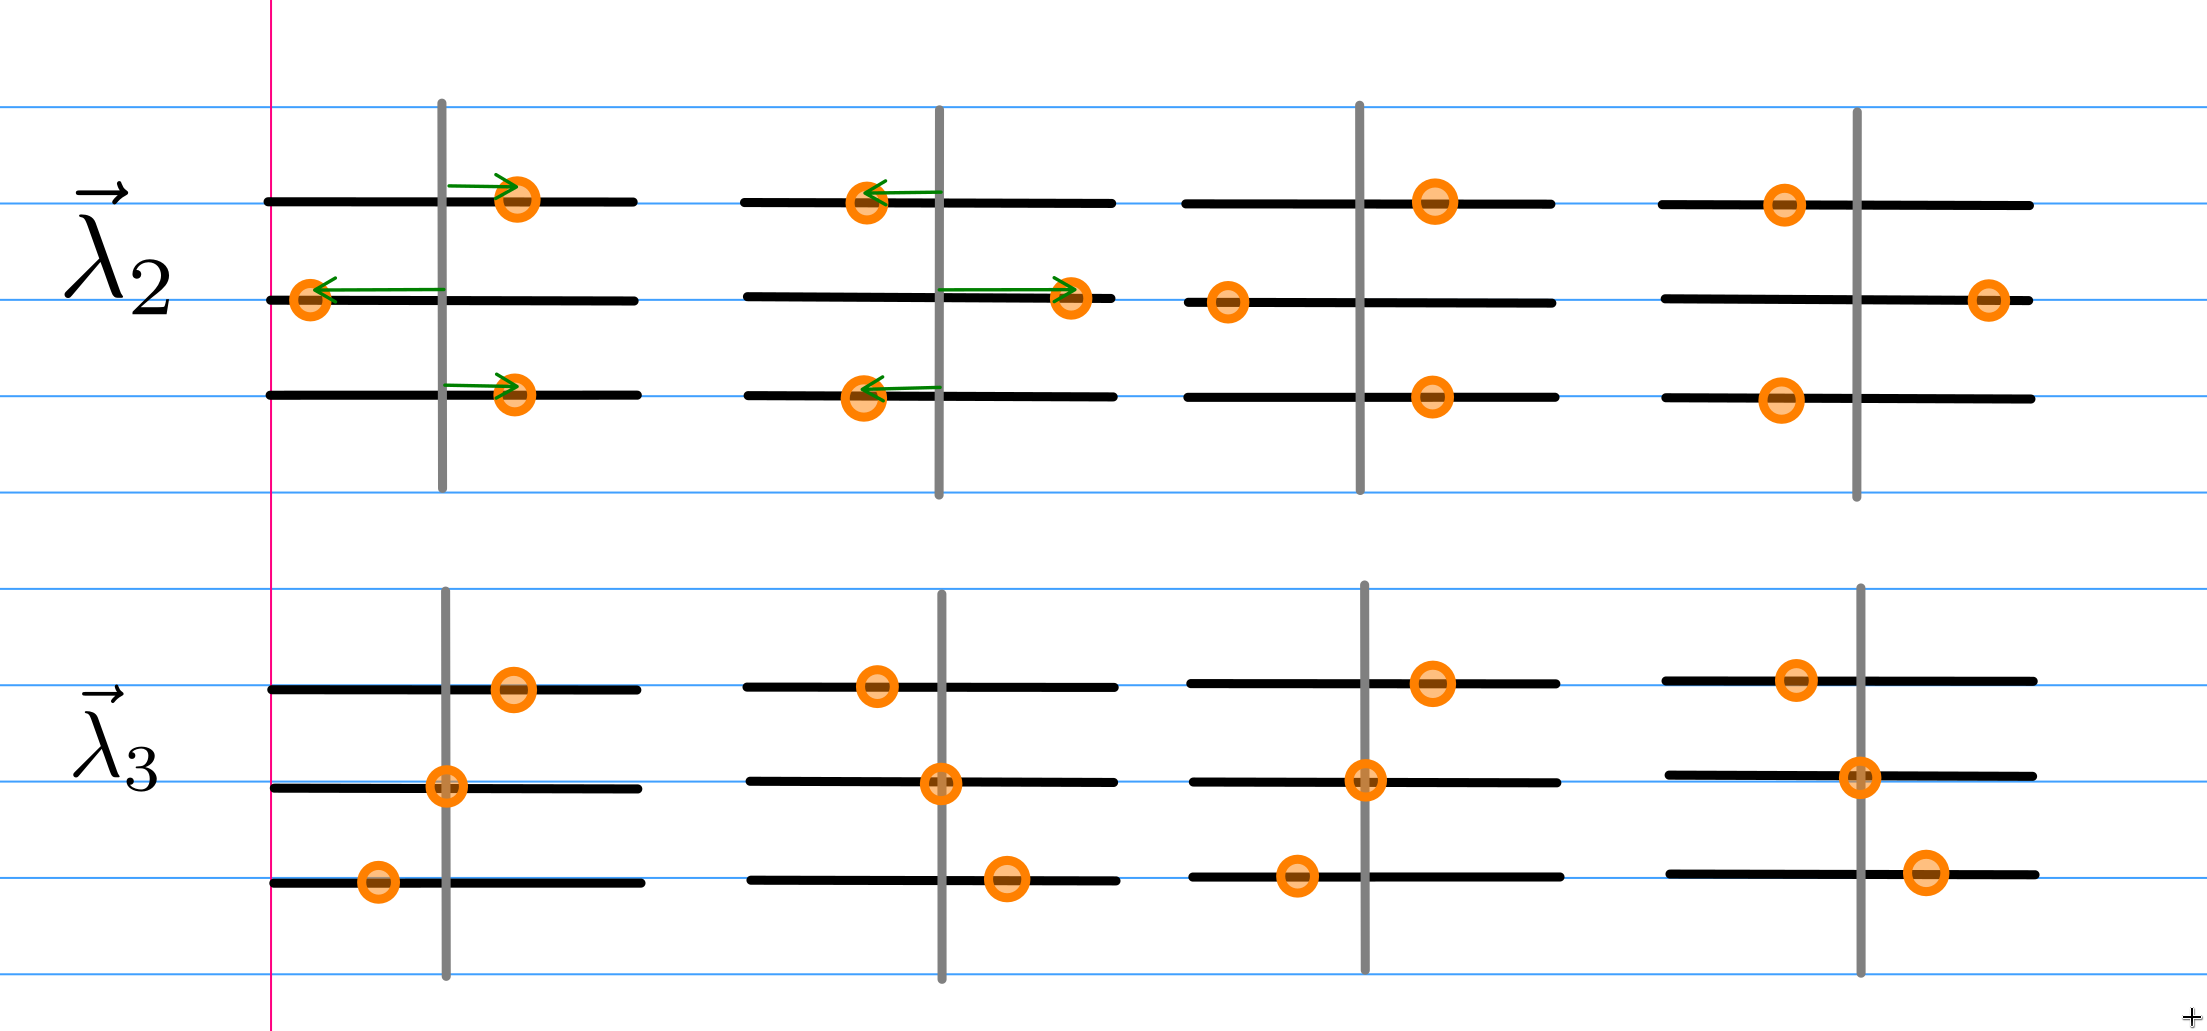
\includegraphics[width=0.8\textwidth]{./ss/11/1.png}
	\caption{./ss/11/1.png}
	\label{fig:-ss-11-1-png}
\end{figure}

For $\vec{\lambda}_2$ is an alternating motion where $\vec{\lambda}_3$ keeps the collinear between 3 particles.



\subsection*{(c)} 

Discussing unstable states, the first possible way how that could occur is if the $\eta$ is too small, so the effects of the middle charge becomes obsolete, then the mutual forces between $1$ and $3$ would be too strong and that can break the equilibrium. It's apparent if we see the eigenfrequency $\omega_3$ where we required $\eta > \frac{1}{4}$ so that $\omega_3^2 > 0$ and not imaginary.

$\eta$ can be indefinitely big (compared to $1$) and still possibly keep the equilibrium. 





\subsection*{(d)} 
Inspired by Morin Chapter 3 on Oscillations we can write the solution in the following way 
\[
\begin{bmatrix} \theta_1 \\ \theta_2 \\\theta_3  \end{bmatrix} 
=
A \begin{bmatrix} 1 \\ - 2 \\ 1 \end{bmatrix} 
\cos(\omega_2 t + \phi_2) +
B \begin{bmatrix} 1 \\ 1 \\ 1 \end{bmatrix}  \] 
Here for $t = 0$ also the speed
\begin{align*}
	\frac{\mathrm{d} }{\mathrm{d}t} 
\begin{bmatrix} \theta_1 \\ \theta_2 \\\theta_3  \end{bmatrix}  = 
A \begin{bmatrix} 1 \\ -2 \\ 1 \end{bmatrix} (- \omega_2) \sin(\omega_2 t + \phi_2) = \vec{0} \implies \phi_2 = 0
\end{align*}
So the cases are  for $t = 0$
\begin{align*}
A \begin{bmatrix} 1 \\ -2 \\ 1 \end{bmatrix} 
+ B \begin{bmatrix} 1\\1\\1 \end{bmatrix}  &=  
\begin{bmatrix} 0 \\ \phi \\ 0 \end{bmatrix}  \\ 
\begin{bmatrix} A  + B \\ 
-2 A  + B \\ 
A + B\end{bmatrix}  &= 
\begin{bmatrix} 0 \\ \phi \\ 0 \end{bmatrix}  \\
\implies A &= - B 
\\
A &= - \frac{\phi}{3}
\end{align*}
Finally
\[
\begin{bmatrix} \theta_1 \\ \theta_2 \\\theta_3  \end{bmatrix} 
=
- \frac{\phi}{3}\begin{bmatrix} 1 \\ - 2 \\ 1 \end{bmatrix} 
\cos(\omega_2 t) 
+ \frac{\phi}{3} \begin{bmatrix} 1 \\ 1 \\ 1 \end{bmatrix}  \] 
Where $\omega_2 = \sqrt{3 \eta k Q^2 / m b^3} $

\newpage
\section*{Problem 05} 
\hrule
Force on any mass, using pure logic of springs 
\begin{align*}
	F_i = - F_{i-1} + F_{i+1} &= -k (\theta_i - \theta_{i-1} ) + k(\theta_{i+1} - \theta_i) \\
				  &= - k \theta_i + k \theta_{i-1} + k \theta_{i+1} - k \theta_i \\
				  &= -2 k \theta_i + k \theta_{i-1} + k \theta_{i+1}  
\end{align*}


\subsection*{(a)} 
\[
	\ddot{\theta}_i = \frac{k}{m} \left(- 2 \theta_i + \theta_{i-1} + \theta_{i+1}\right)
\]


\subsection*{(b)} 
The chain of equation are 
\begin{align*}
	F_1 &= - 2 k \theta_1 + k \theta_N + k \theta_2 \\ 
F_2 &=  - 2 k \theta_2 + k \theta_1 + k \theta_3 \\
F_3 &= - 2 k \theta_3 + k \theta_2 + k \theta_4  \\
    & \vdots \\  
F_{N-1} &= - 2 k \theta_{N-1} + k \theta_{N-2} + k \theta_{N} \\
F_N &= - 2 k \theta_N + k \theta_{N-1} + k \theta_1 \\
\end{align*}
Finding the matrix representation 
\[
\begin{bmatrix} F_1 \\ F_2 \\ F_3 \\ \vdots \\ F_N \end{bmatrix}  = 
\begin{bmatrix}
	-2k & k & 0 & 0 & \cdots & 0 & k \\ 
	k & -2k & k & 0 & \cdots & 0 & 0 \\ 
	0 & k & -2k & k & \cdots & 0 & 0 \\ 
	\vdots & 
	\vdots & 
	\vdots & 
	\vdots & 
	\ddots & 
	\vdots & 
	\vdots \\ 
	k& 0 & 0 & 0 & \cdots & k & -2k \\ 
\end{bmatrix} 
\begin{bmatrix} \theta_1 \\ \theta_2 \\ \theta_3 \\ \vdots \\ \theta_N \end{bmatrix} 
\] 
This can be written as 
\[
\begin{bmatrix} F_1 \\ F_2 \\ F_3 \\ \vdots \\ F_N \end{bmatrix}  = 
- k 
\begin{bmatrix}
	2 & -1 & 0 & 0 & \cdots & 0 & -1 \\ 
	-1 & 2 & -1 & 0 & \cdots & 0 & 0 \\ 
	0 & -1 & 2 & -1 & \cdots & 0 & 0 \\ 
	\vdots & 
	\vdots & 
	\vdots & 
	\vdots & 
	\ddots & 
	\vdots & 
	\vdots \\ 
	-1& 0 & 0 & 0 & \cdots & -1 & 2 \\ 
\end{bmatrix} 
\begin{bmatrix} \theta_1 \\ \theta_2 \\ \theta_3 \\ \vdots \\ \theta_N \end{bmatrix} 
\] 
Focusing on the matrix 
\[
\begin{bmatrix}
	2 & -1 & 0 & 0 & \cdots & 0 & -1 \\ 
	-1 & 2 & -1 & 0 & \cdots & 0 & 0 \\ 
	0 & -1 & 2 & -1 & \cdots & 0 & 0 \\ 
	\vdots & 
	\vdots & 
	\vdots & 
	\vdots & 
	\ddots & 
	\vdots & 
	\vdots \\ 
	-1& 0 & 0 & 0 & \cdots & -1 & 2 \\ 
\end{bmatrix}  
= 3 I - 
\begin{bmatrix} 1 & 1 & 0 & 0 & \cdots & 1 \\ 
1 & 1 & 1 & 0 & \cdots & 0 \\ 
0 & 1 & 1 & 1 & \cdots & 0 \\ 
	\vdots & 
	\vdots & 
	\vdots & 
	\vdots & 
	\ddots & 
	\vdots \\ 
	1 & 0 & 0 & 0 &  \cdots & 1  
\end{bmatrix}  = 3 I - \mathcal M 
\] 

We are interested on this $\mathcal M$.

\begin{itemize}
	\item The cyclic nature of $\mathcal M$ can give us some motivation to guess the eigenvectors. We will attack this problem with Polynomials.\footnote{This problem was part of my self-study before going to International Physics Olympiad so there's a lot of nostalgia attached to this funny matrix.}
	\item I searched up for some papers that deals with this problem, here's one for alternating signs and general case
\href{https://www.sciencedirect.com/science/article/pii/S0024379513005776}{[Paper 1 Link]} 
\item Inspired, we will look at the $N$-th root of $1$ which is $\eta.$ I take assistance from MATH 382 Computation Complex Analysis courework where the $N$-th root $\eta$ $n$-th term can be given by $\eta_n = \exp(2 \pi i n / N)$ and obviously $0 \le n < N$. 
\item Given the condition of $\eta$, \[
\begin{bmatrix} 1 \\ \eta \\ \eta^2 \\ \vdots \\ \eta^{N-1} \end{bmatrix} 
\] is an eigenvector with eigenvalue $\eta ^{-1} + 1 + \eta $ in this case.  
\item The eigenvalues of the entire matrix $3 I - \mathcal M$ hence are given by  $3 - (\eta ^{-1} + 1 + \eta ) = 2 - \eta^{-1} - \eta$. 
\item Because of $N$ different roots of $1$ as given by $\eta_n$, the eigenvalues are for $0 \le n < N$ 
	\[
	\lambda_n = 2 - \eta^{-1}_n - \eta_n = 2 - \left(e^{- 2 \pi i n / N} + e^{ 2 \pi i n / N}\right)
	\]
	Turning to cosines 
	\[
	\lambda_n = 2 - 2 \cos (2 \pi n / N ) \implies \lambda_n = 4 \sin ^2 (\pi n / N )
	\]
	And the corresponding eigenvector is 
	\[ \ket{4 \sin ^2 (\pi n / N)} = 
	\begin{bmatrix} 1 \\ \eta_n \\ \eta^2_n \\ \vdots \\ \eta^{N-1}_n  \end{bmatrix} 
	\] 
\item Since the numbers $n$ and $N-n$ yield the same value for $\lambda_n$ in $4 \sin ^2 (\pi n / N)$, the eigenvalues tend to come in pairs (except for when $n = 0$ and $n = N / 2$ if $N$ is even). Because of this we can form real linear combinations of the two corresponding complex eigenvectors given in $\begin{bmatrix} 1 & \eta_n & \eta^2_n & \cdots & \eta^{N-1}_n  \end{bmatrix} $. 

\item The two vectors 
	\[
		V^{+}_n = \frac{1}{2} \left(V_n + V_{N-n}\right) = 
		\begin{bmatrix} 1 \\ 
		\cos(2 \pi n  / N) \\ 
	\cos (4 \pi n / N) \\ 
\vdots 
\\
\cos (2 (N-1) \pi n / N )\end{bmatrix} 
	\] 
	\textbf{and}
	\[
		V^{-}_n = \frac{1}{2 i} (V_n - V_{N-n}) = 
		\begin{bmatrix} 0 \\ 
		\sin(2 \pi n / N) \\ 
	\sin (4 \pi n / N ) \\ 
\vdots 
\\ 
\sin(2 (N-1) \pi n / N)\end{bmatrix} 
\] both have eigenvalue $\lambda_n = \lambda_{N-n}$ as discussed in the last itemized point. Note that we see \textbf{degeneracy} here. 
\item Eigenfrequency corresponding to the two above normal modes are 
	\[
		\lambda_n = 4 \sin ^2 (\pi n  / N) \implies\omega_n = \sqrt{ \frac{k}{m}} (2 \sin (\pi n / N))
	\] 
\end{itemize}



\subsection*{(c)}
\[
\omega_n = 2 \sqrt{\frac{k}{m}} \sin(\pi n / 4)
\] 
For $N =4$, if $n= 0$ we find $\lambda_0 =\omega_0= 0$ and $V_0 = (1,1,1)$.

For $n = 1$ we find $\lambda_1 = \sqrt{k / m}   2 \sin(\pi /4 ) = \sqrt{2}  \sqrt{k / m}  $. Modes
\begin{align*}
	V^{+}_4 &= 
		\begin{bmatrix} 1 \\ 
		\cos(2 \pi n  / 4) \\ 
	\cos (4 \pi n / 4) \\ 
\cos (6 \pi n / 4 )\end{bmatrix} 
		\\
	V^{-}_4 &= 
		\begin{bmatrix} 0 \\ 
		\sin(2 \pi n / 4) \\ 
	\sin (4 \pi n / 4 ) \\ 
\sin(6 \pi n / 4)\end{bmatrix} 
\end{align*}

\begin{align*}
	V^{+}_4 &= 
		\begin{bmatrix} 1 \\ 
		\cos(2 \pi   / 4) \\ 
	\cos (4 \pi / 4) \\ 
\cos (6 \pi  / 4 )\end{bmatrix}  
= 
	\begin{bmatrix} 1\\ 0 \\ -1 \\ 0 \end{bmatrix} 
		\\
	V^{-}_4 &= 
		\begin{bmatrix} 0 \\ 
		\sin(2 \pi  / 4) \\ 
	\sin (4 \pi  / 4 ) \\ 
\sin(6 \pi / 4)\end{bmatrix} 
=
\begin{bmatrix} 0 \\ 1 \\ 0 \\ -1 \end{bmatrix} 
\end{align*}

For $n = 2$ we find we find $\omega_2 = 2 \sqrt{k / m} $


\begin{align*}
	V^{+}_4 &= 
		\begin{bmatrix} 1 \\ 
		\cos(2 \pi   / 2) \\ 
	\cos (4 \pi / 2) \\ 
\cos (6 \pi  / 2 )\end{bmatrix}  
= 
	\begin{bmatrix} 1\\ -1 \\ 1 \\ -1 \end{bmatrix} 
		\\
	V^{-}_4 &= 
		\begin{bmatrix} 0 \\ 
		\sin(2 \pi  / 2) \\ 
	\sin (4 \pi  / 2 ) \\ 
\sin(6 \pi / 2)\end{bmatrix} 
=
\begin{bmatrix} 0 \\ 0 \\ 0 \\ 0 \end{bmatrix} 
\end{align*}



For $n = 3$ we find $\omega_3 = \sqrt{2} \sqrt{k / m} $. This will give the same eigenvectors as we had seen that $n$ and $N - n$ are the same. So $n = 1$ and $N - 1 = 3$ will be the same case. Same for $n = 4$ where $\omega_4 = 2 \sqrt{k / m}  $ .

So the eigenmodes are (where degeneracy is present with two different eigenmodes for one eigenfrequency)
\[
	\text{for }  \sqrt{2 k / m}  \implies 
\begin{bmatrix} 0 \\ 1 \\ 0 \\ -1 \end{bmatrix} 
\text{ and }
	\begin{bmatrix} 1\\ 0 \\ -1 \\ 0 \end{bmatrix} 
\]
\begin{figure}[H]
	\centering
	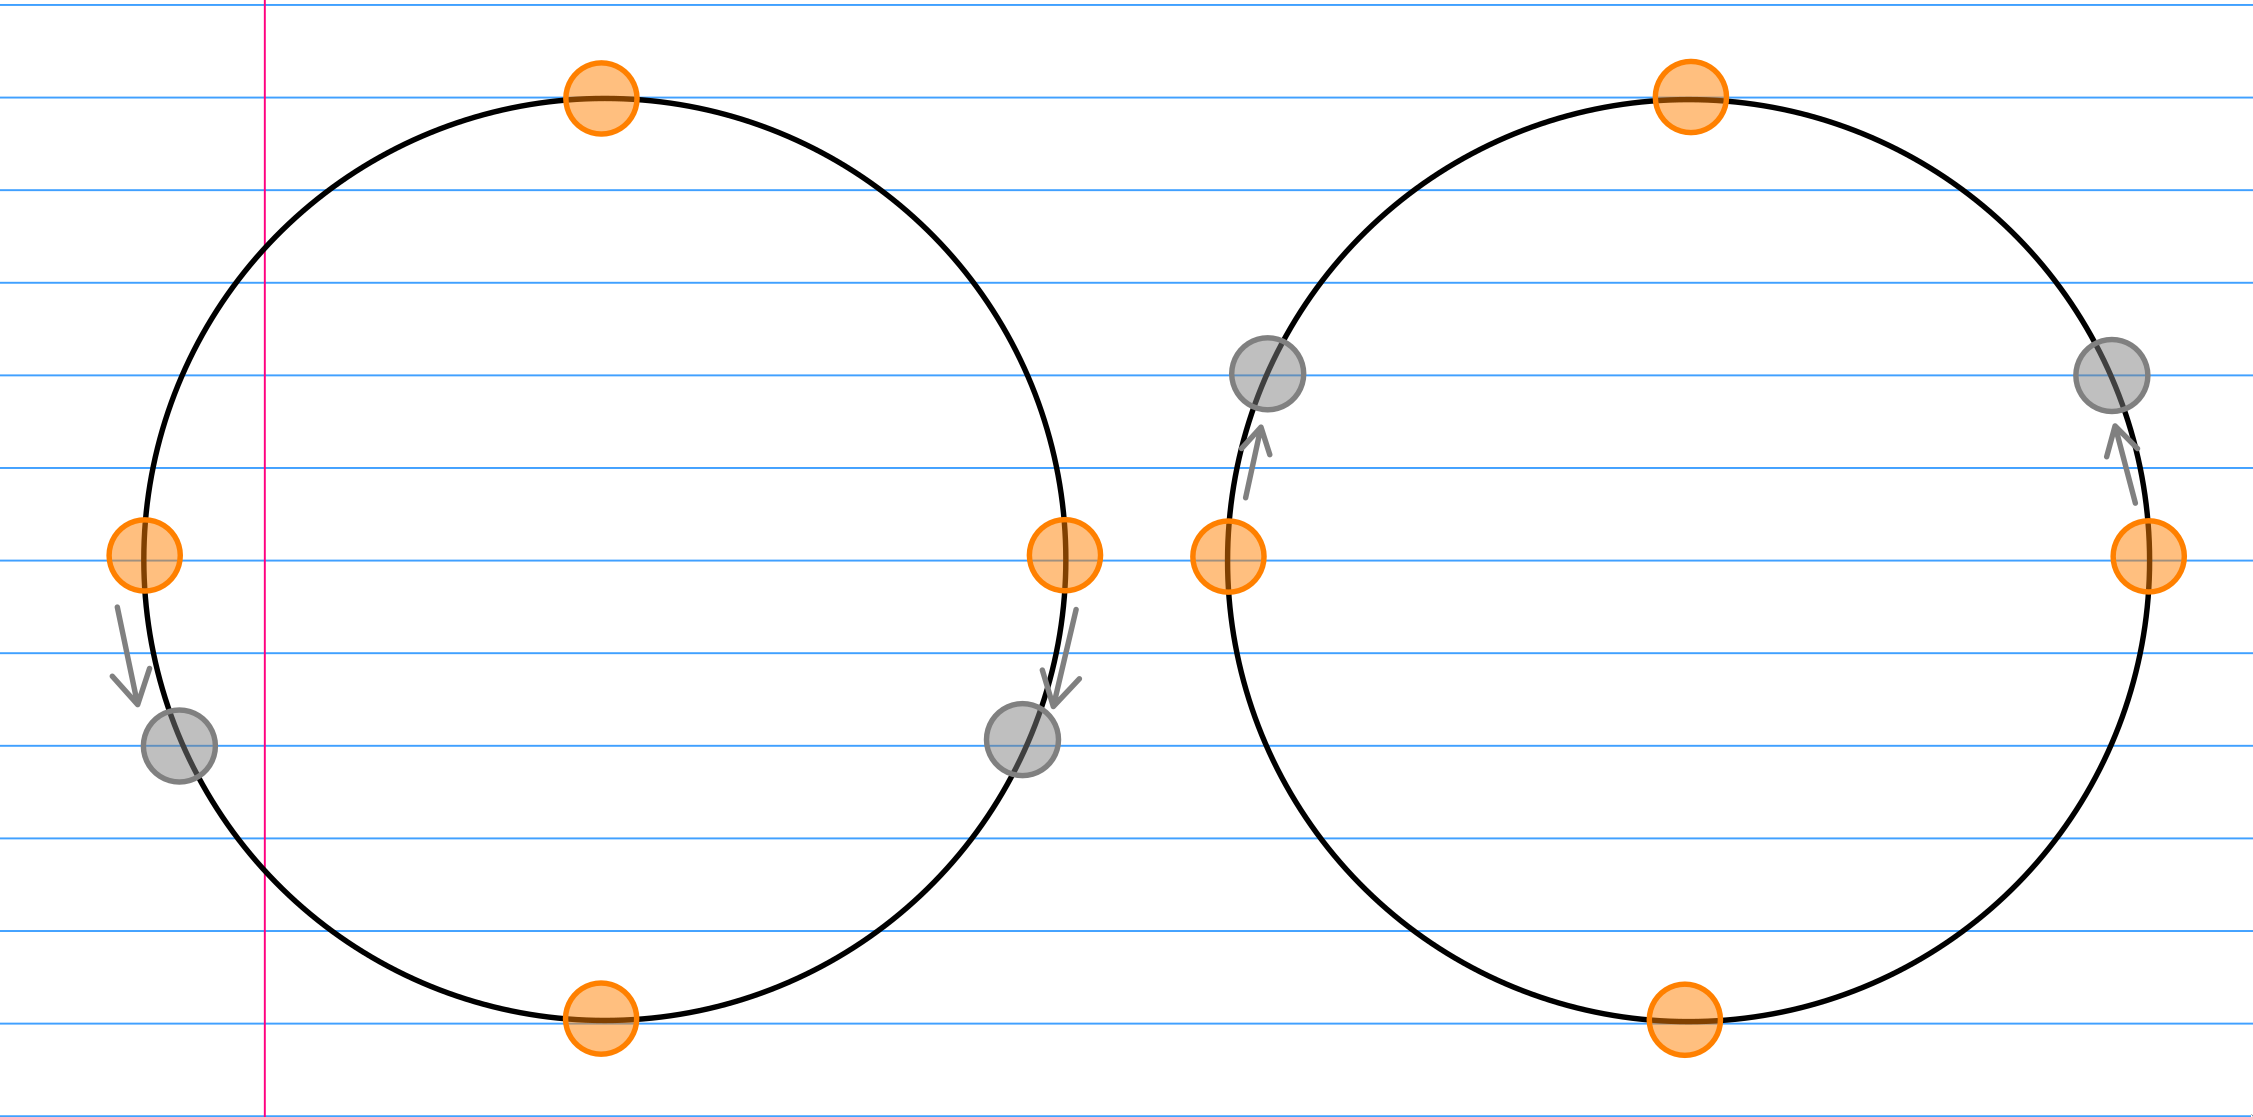
\includegraphics[width=0.8\textwidth]{./ss/11/2.png}
	\caption{The mode $(0,1,0,-1)$}
	\label{fig:-ss-11-2-png}
\end{figure}
\begin{figure}[H]
	\centering
	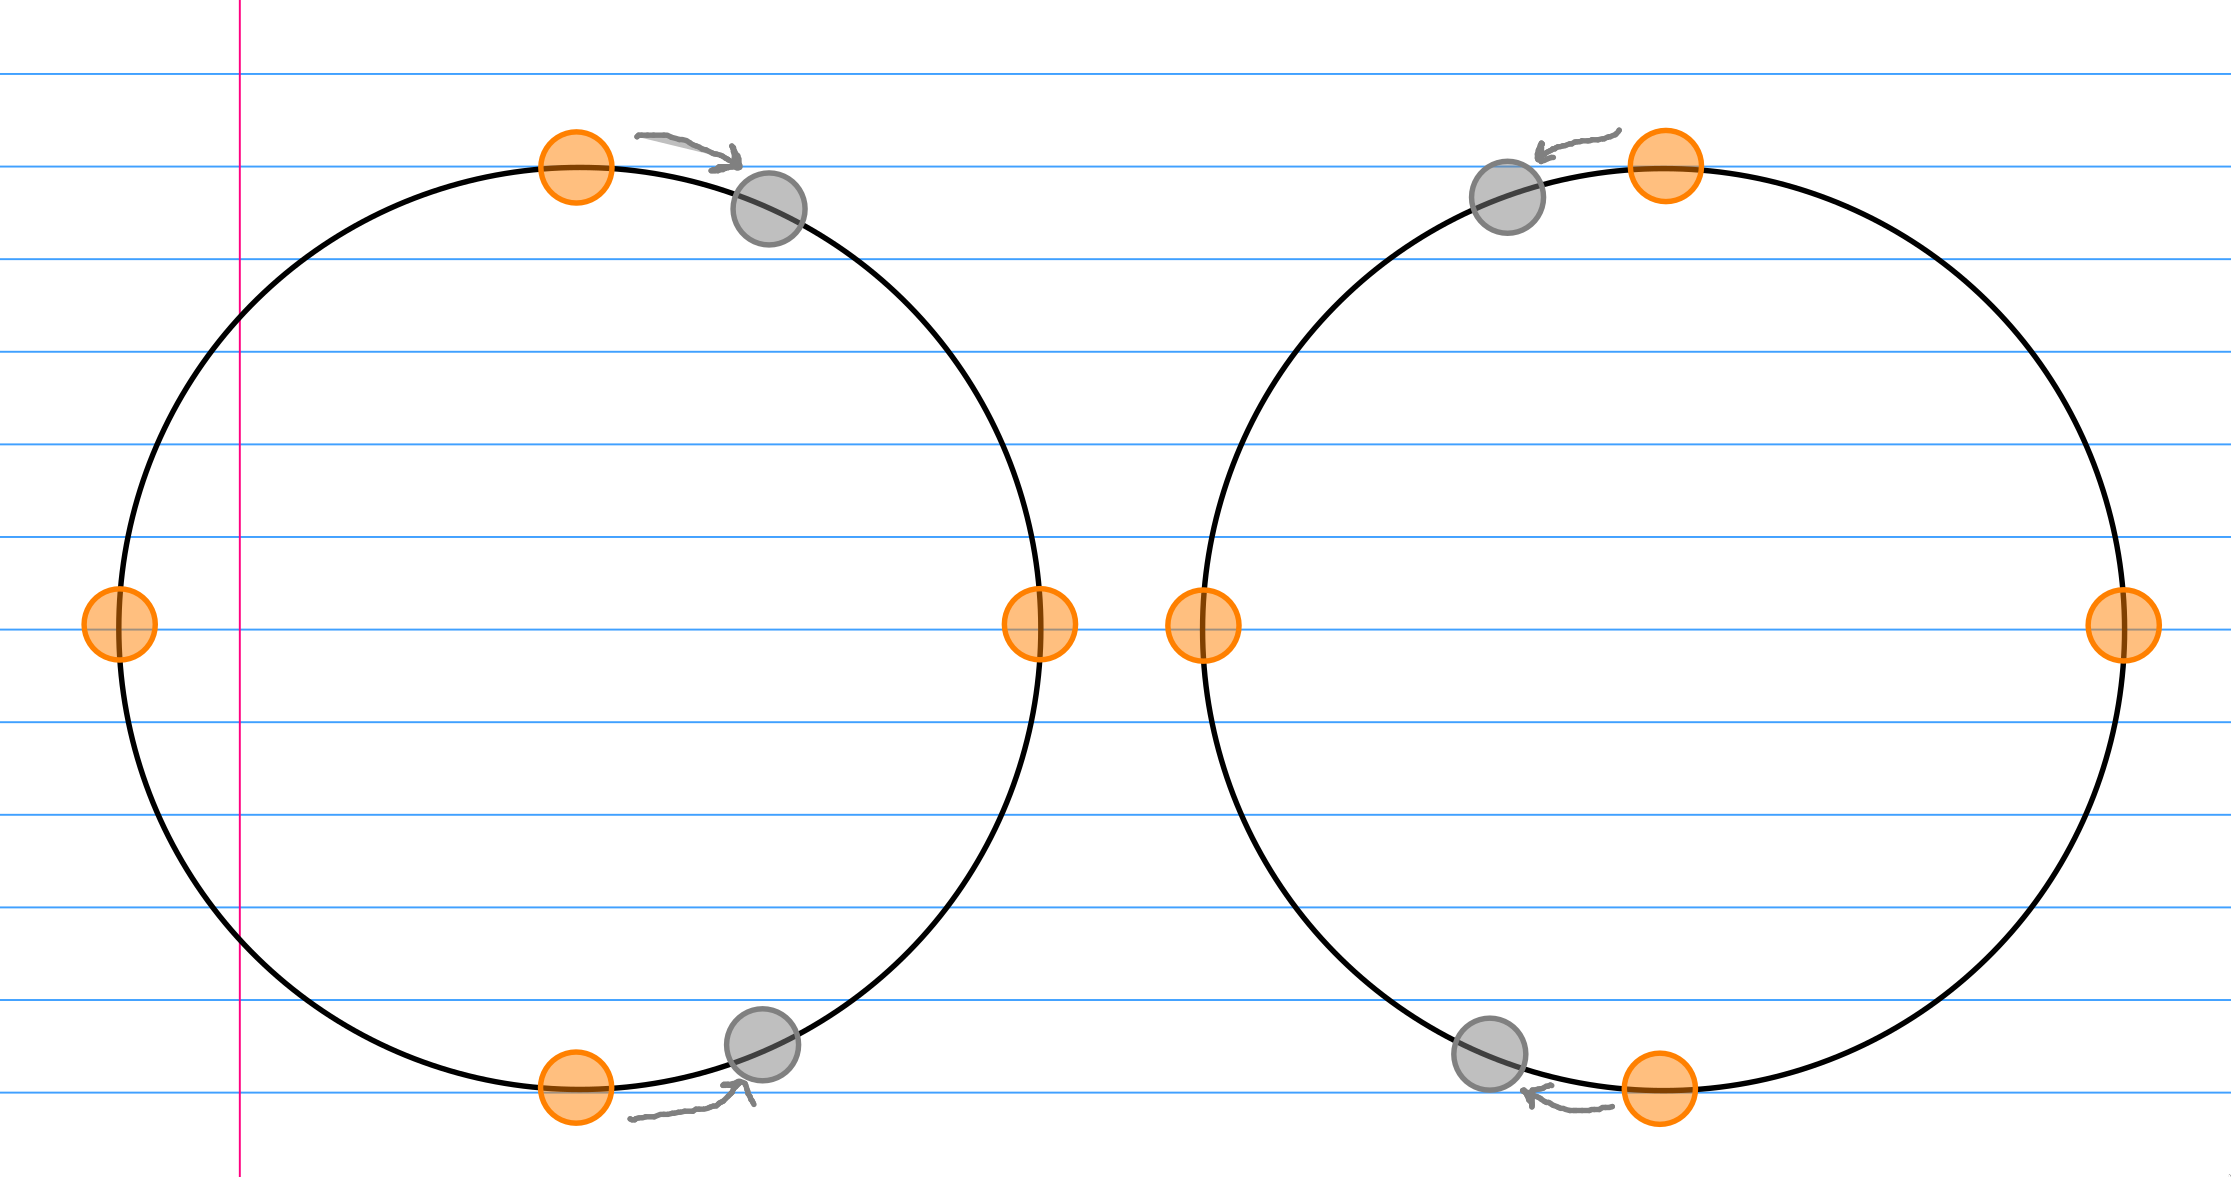
\includegraphics[width=0.8\textwidth]{./ss/11/3.png}
	\caption{The mode $(1,0,-1,0)$}
	\label{fig:-ss-11-3-png}
\end{figure}
\[
\text{for } 2\sqrt{k / m}  \implies 
	\begin{bmatrix} 1\\ -1 \\ 1 \\ -1 \end{bmatrix} \text{ and }
\begin{bmatrix} 0 \\ 0 \\ 0 \\ 0 \end{bmatrix} 
\] 
\begin{figure}[H]
	\centering
	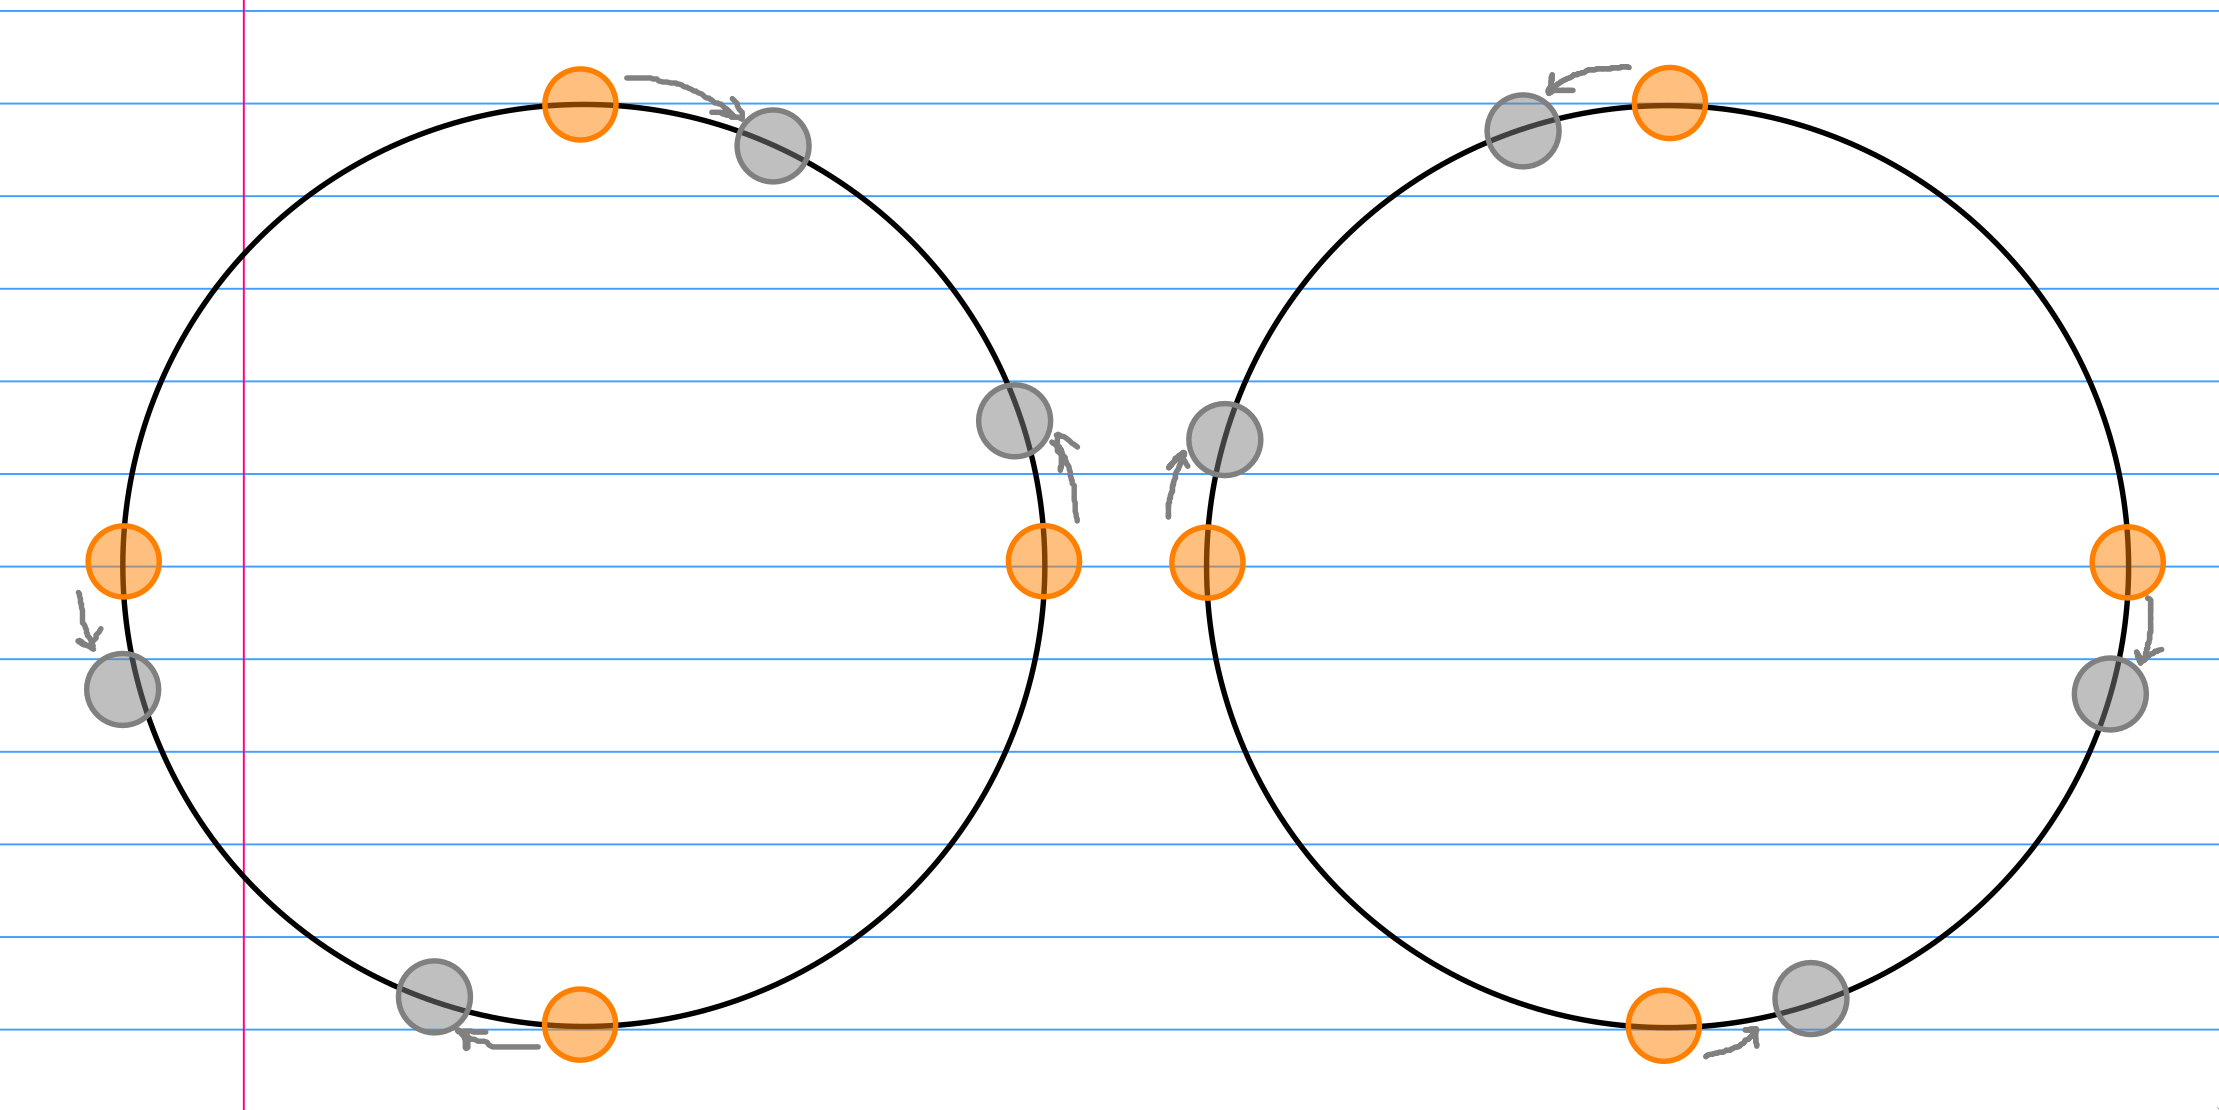
\includegraphics[width=0.8\textwidth]{./ss/11/4.png}
	\caption{The mode for $(1,-1,1,-1)$}
	\label{fig:-ss-11-4-png}
\end{figure}




















\newpage 
\section*{Problem 5}
\hrule 




\subsection*{(a)}
\subsection*{\emph{Studying the problem}}
The initial configuration of the string 
\[
q(x,0) = f(x) = 
\begin{cases}
	\frac{2h}{L}x & 0 \le x \le \frac{L}{2} \\
	2h - \frac{2h}{L}x & \frac{L}{2} \le  x \le  L 
\end{cases}
\]
\[
	\frac{\partial q(x,t)}{\partial t} _{t=0} = \sum_{n=1}^{\infty} d_n \Omega_n \phi_n(x) = g(x) = 0 \implies \boxed{
	d_n = 0
	} 
\] 
The general solution to the string equation (assumed solution is separable between time and position)
\[
	q(x,t) = \sum_{n=1}^{\infty} [c_n \cos(\Omega_n t) + d_n \sin(\Omega_n t) ] \phi_n(x)
\]
For $t = 0$ we get, 
\[
	q(x,0) = f(x) = \sum_{n=1}^{\infty} c_n \phi_n(x)\] 
We are interested on finding the general solution of $q(x,t)$ that will hold for the future given this initial condition. The variables of our equation are obviously $x,t$ and what we need to find out is $c_n, d_n$. The next sub-section will find out a solution for $c_n$ ($d_n$ is trivially zero given zero initial velocity).



\subsection*{\emph{Solving for $c_n$} }
Let us do the following computation now. Let us multiply both sides of the above equation with $\phi_p(x)$ where $p$ represents the  $p$-th term while we take a summation over the index of $n$.
\[
f(x) \phi_p (x) = \sum_{n=1}^{\infty} c_n \phi_n(x) \phi_p(x)
\]
Just so that we can invoke the inner product between orthonormal bases, we can take an integral with the following way
\begin{align*}
	\int_{0}^{L} \mathrm{d} x \,  f(x) \phi_p(x) =& \int_{0}^{L} \mathrm{d} x\,  \left(
 \sum_{n=1}^{\infty} c_n \phi_n(x) \phi_p(x) \right) \\ 
		=& \sum_{n=1}^{\infty} c_n \int_{0}^{L} \mathrm{d} x \, \phi_n(x) \phi_p(x)  \\
		=& \sum_{n=1}^{\infty} c_n \delta_{np} \frac{L}{2} \\
		=& c_p \frac{L}{2}
\end{align*}
This above gives us the $p$-th term
\[
c_p = \frac{2}{L} \int_{0}^{L} \mathrm{d} x \, f(x) \phi_p(x)  
\] 
Using the explicit equation for the bases and also looking at the piecewise function, we can write, 
\begin{align*}
	c_p &= \frac{2}{L} \int_{0}^{L} \mathrm{d} x \, f(x) \sin \left( \frac{p \pi x }{L}\right)  \\
	&= \frac{2}{L} 
	\left( \int_{0}^{\frac{L}{2}}  f(x) \sin\left(\frac{p \pi x}{L}\right) + 
	\int_{\frac{L}{2}}^{L} f(x) \sin \left(\frac{p \pi x}{L}\right)  \right)\\
	&= \frac{2}{L} 
	\left(
	\int_{0}^{\frac{L}{2} } \frac{2h}{L} x \sin\left(\frac{p \pi x}{L}\right) +
	\int_{\frac{L}{2}}^{L} \left(2 h - \frac{2h}{L} x \right) \sin \left(\frac{p \pi x}{L}\right) 
	\right)\\
	&= 
	\frac{2}{L} 
	\left(
\frac{hL}{\pi ^2 p^2 } \left[ 
2 \sin \left(p \frac{\pi}{2} \right) - \pi p \cos \left(p \frac{\pi}{2}\right)
\right]  - \frac{hL}{\pi ^2 p ^2} 
\left[
	2 \sin\left(\pi p \right) - 2 \sin \left(p \frac{\pi}{2}\right) - \pi p \cos \left(p \frac{\pi}{ 2}\right)
\right]
	\right)\\ 
	&= \frac{8h}{\pi ^2 p^2} \sin \left(p \frac{\pi}{2}\right) \left[1 - \cos \left(p \frac{\pi}{2}\right)\right] \\
\end{align*}
Hence if I write this huge mess properly
\[
\boxed{
	c_p = \frac{8h}{\pi ^2 p ^2} \sin\left(\frac{p \pi }{2}\right) \left[ 1 - \cos \left(\frac{p \pi }{2}\right) \right]
}
\] 



\subsection*{\emph{Discussion on odd and even modes}}
\begin{figure}[H]
	\centering
	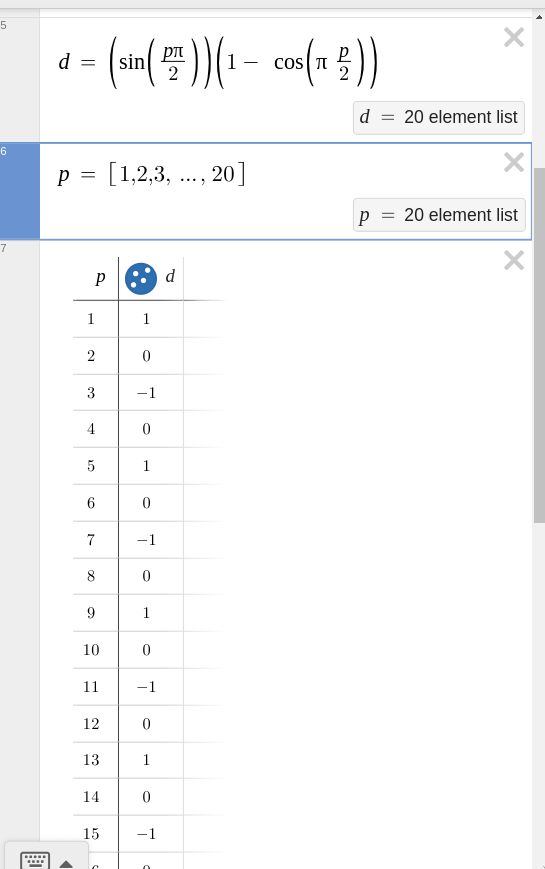
\includegraphics[width=0.6\textwidth]{../phys311/ss/graph-cn.png}
	\caption{ss/graph-cn.png}
	\label{fig:ss-graph-cn-png}
\end{figure}
We can see that every \emph{even} numbers is giving us a $0$ for $c_p$ ($d$ term in graph). The \emph{odd} terms alter between $-1$ and $1$. The contribution of even and odd modes is obvious from here.   
\subsection*{\emph{Plotting the displacement with time}}
Let's set $L = 1$ and we will look at $0 \le  x \le 1$. 

As given $\Omega_n = k_n = \frac{n\pi}{L} = n \pi $. 

For $h$ let's pick $h = 0.4$. 

Using hte $c_p$ we derived above, the displacement function $q(x,t)$ is then, 
\[
	q(x,t)_{(10)}= 
\sum_{n=1}^{10} c_n \cos ( n \pi t) \sin(n \pi x)
\] 
Expanding $c_n$, 
\[
q(x,t)_{(10)} = \frac{8 (0.4)}{\pi ^2} 
\sum_{n=1}^{10} 
\frac{1}{n^2} \sin \left(\frac{n \pi }{2}\right) 
\left[ 
1 - \cos \left(\frac{n \pi }{2}\right)
\right] 
\cos \left( n \pi t\right) \sin (n \pi x)
\]
And $\tau = \frac{2\pi}{\Omega_1} = \frac{2 \pi }{\pi } = 2$


The first three non zero terms of the sum are 
\[
\frac{8h}{\pi ^2 }
\left(
\cos(\pi t) \sin(\pi x) 
+
\left(-\frac{1}{9}\right) \cos(3 \pi t) \sin (3 \pi x)
+ 
\left(\frac{1}{25}\right) \cos(5 \pi t) \sin(5 \pi t)
\right)
\] 

\newpage

\begin{center}
	{\huge \textbf{Plots of $q(x,t)$ where $\tau = 2$ }}
\end{center}
\[
\boxed{
q(x,t)_{(10)} = \frac{8 (0.4)}{\pi ^2 } 
\sum_{n=1}^{10} \frac{1}{n^2} \sin \left(\frac{n \pi }{2}\right) 
\left[ 
1 - \cos \left(\frac{n \pi }{2}\right)
\right] \cos \left( n \pi t\right) \sin (n \pi x) 
\quad \text{and } x \in [0,1]
}\]
\begin{minipage}{0.5\textwidth}
\begin{figure}[H]
	\centering
	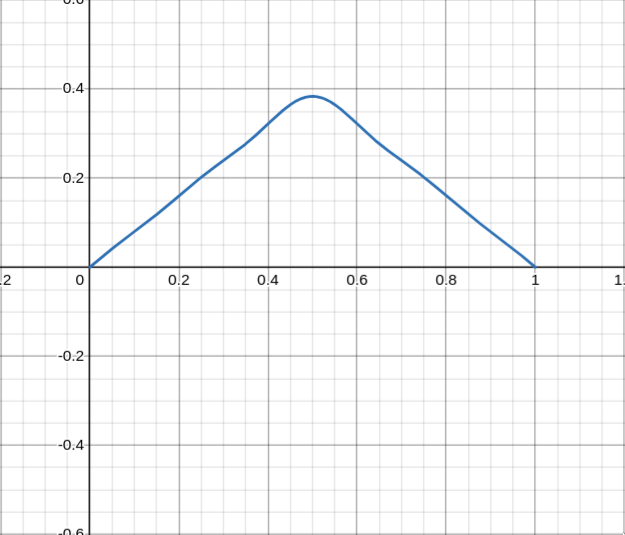
\includegraphics[width=0.9\textwidth]{../phys311/ss/c_n_001.png}
	\caption{$t = 0$ and also $t = \tau$}
	\label{fig:ss-c_n_001-png}
\end{figure}
\begin{figure}[H]
	\centering
	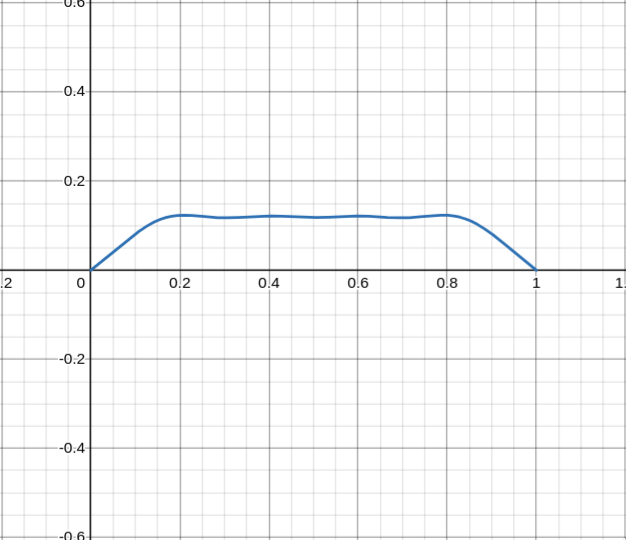
\includegraphics[width=0.9\textwidth]{../phys311/ss/c_n_025.png}
	\caption{$t = 0.35$}
	\label{fig:ss-c_n_01-png}
\end{figure}
\end{minipage}
\hfill %
\begin{minipage}{0.5\textwidth}
\begin{figure}[H]
	\centering
	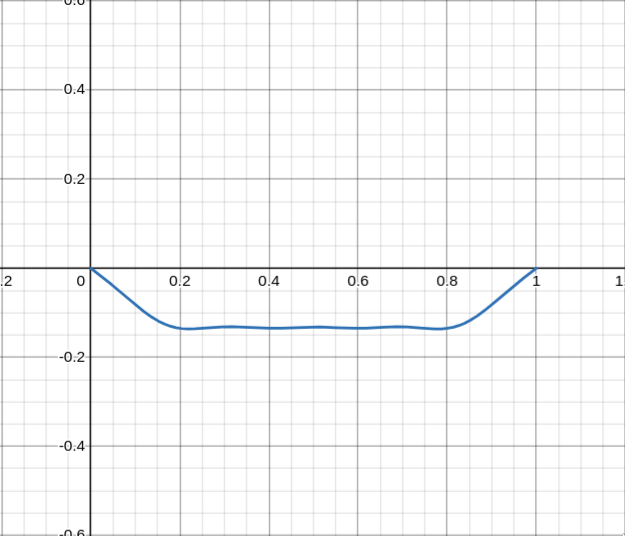
\includegraphics[width=0.9\textwidth]{../phys311/ss/c_n_02.png}
	\caption{$t = \frac{\tau}{3} = \frac{2}{3}$}
	\label{fig:ss-c_n_01-png}
\end{figure}
\begin{figure}[H]
	\centering
	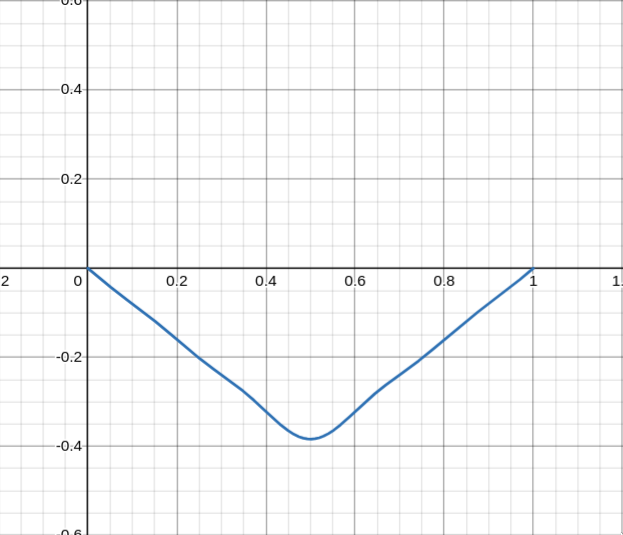
\includegraphics[width=0.9\textwidth]{../phys311/ss/c_n_03.png}
	\caption{$t = \frac{\tau}{2} = 1$}
	\label{fig:ss-c_n_01-png}
\end{figure}
\end{minipage}
\newpage



\subsection*{(b)}
\subsection*{\emph{Studying the Problem}}
Initially the string is tight and straight hence 
\[
q(x, 0) = \sum_{n=1}^{\infty} c_n \phi_n(x) = f(x) = 0 \implies \boxed{
c_n = 0
}
\] 
\[
	\frac{\partial q(x,t)}{\partial t} _{t = 0} = g(x) = v_0 \theta\left(a - \left|x - \frac{L}{2} \right|\right)
\]
Where $\theta(x)$ is a Heaviside step function (outputs 1 whenever input is 0 or positive).
I am not going to waste my and graders time by re-writing everything I wrote above, the procedure we are going to follow is same as above. 

\subsection*{\emph{Computation of $d_n$ }}
\begin{align*}
	g(x) &= \sum_{n=1}^{\infty} d_n \Omega_n \phi_n(x)   \\
\int_{0}^{L} \mathrm{d} x\, 	g(x) \phi_p (x) &= \sum_{n=1}^{\infty}  \int_{0}^{L} \mathrm{d} x \, d_n \Omega_n \phi_n (x) \phi_p (x)\\
\int_{\frac{L}{2} - a}^{\frac{L}{2} + a} v_0 \phi_p (x) &= d_p  \Omega_p \frac{L}{2} \\ 
\int_{\frac{L}{2}- a}^{\frac{L}{2} + a} v_0 \sin (k_p x) &= d_p  k_p \frac{L}{2}\\ 
\frac{v_0}{k_p} \left[ - \cos \left(k_p x\right)\right]_{x = \frac{L}{2} - a}^{x = \frac{L}{2}+a} &= d_p k_p \frac{L}{2} \\ 
\cos \left(k_p \frac{L}{2} - k_p a\right)- \cos \left( k_p \frac{L}{2} + k_p a\right)  &= \frac{d_p k_p^2 L}{2v_0} \\
\cos \left( \frac{n \pi }{2} - \frac{n \pi a}{L}\right) - 
\cos \left( \frac{n \pi }{2} + \frac{n \pi a}{L}\right) &= \frac{d_p n^2 \pi ^2 }{2 v_0 L} \\ 
\end{align*}
This gives us 
\[
d_p = \frac{2 v_0 L}{n^2 \pi ^2} 
\left[ 
\cos \left( \frac{n \pi }{2} - \frac{n \pi a}{L}\right) - 
\cos \left( \frac{n \pi }{2} + \frac{n \pi a}{L}\right) 
\right] 
= \frac{4 v_0 L}{n^2 \pi ^2} \sin \left(\frac{n \pi }{2}\right) \sin \left(\frac{n \pi a}{L}\right)
\]

\subsection*{\emph{Discussion on Even and Odd modes}}
\begin{figure}[H]
	\centering
	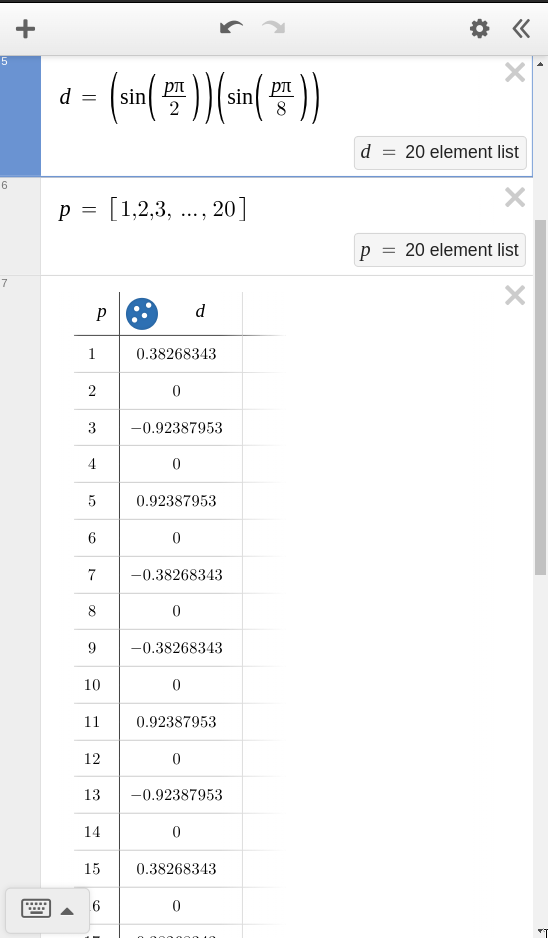
\includegraphics[width=0.6\textwidth]{../phys311/ss/graph-dn}
	\caption{ss/graph-dn}
	\label{fig:ss-graph-dn}
\end{figure}
Like before we can see every  \emph{even} modes are 0. 

The first three terms of the expansion 
\[
\frac{4v_0 L}{\pi^2} \left(
	(0.382)\sin(\pi t)\sin(\pi x) + 
	(-0.923)\sin(3 \pi t) \sin(3 \pi x)+ 
	(0.923) \sin(5 \pi t) \sin(5 \pi x) 
\right)
\] 
\newpage 
\begin{center}
	{\huge \textbf{Plots of $q(x,t)$ where $\tau = 2$ }}
\end{center}
\[
\boxed{
q(x,t)_{(10)} = \frac{4 (1.5)}{\pi ^2} 
\sum_{n=1}^{10} \frac{1}{n^2}
\sin \left( \frac{n \pi }{2}\right) \sin \left({n \pi (1 / 8)}\right) 
\sin \left( n \pi t\right) \sin \left(n \pi x\right)
\quad \text{and } x \in [0,1]
}\]
\begin{minipage}{0.5\textwidth}
\begin{figure}[H]
	\centering
	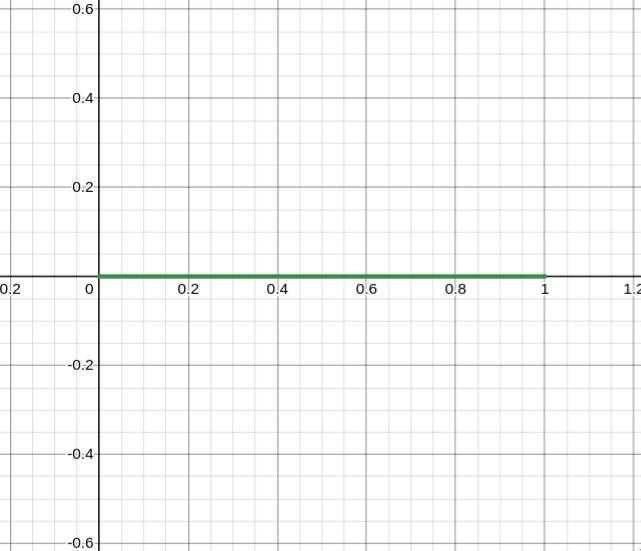
\includegraphics[width=0.9\textwidth]{../phys311/ss/d_n_03.png}
	\caption{$t = 0$ and also $t = \tau$}
	\label{fig:ss-c_n_001-png}
\end{figure}
\begin{figure}[H]
	\centering
	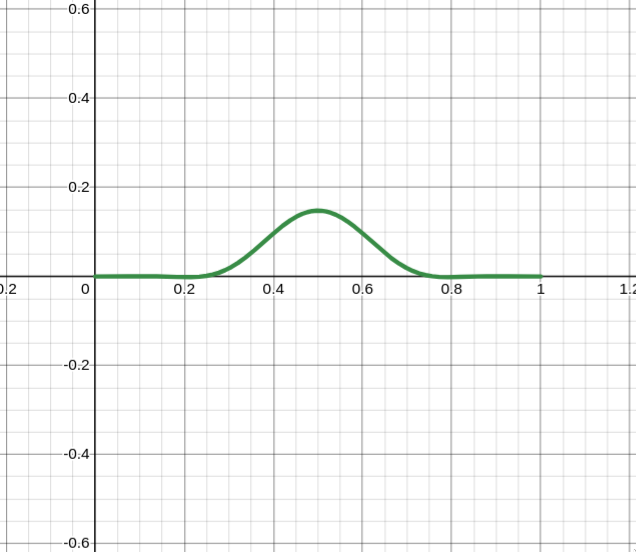
\includegraphics[width=0.9\textwidth]{../phys311/ss/d_n_025.png}
	\caption{$t = \frac{\tau}{20} = 0.1 $}
	\label{fig:ss-c_n_01-png}
\end{figure}
\end{minipage}
\hfill %
\begin{minipage}{0.5\textwidth}
\begin{figure}[H]
	\centering
	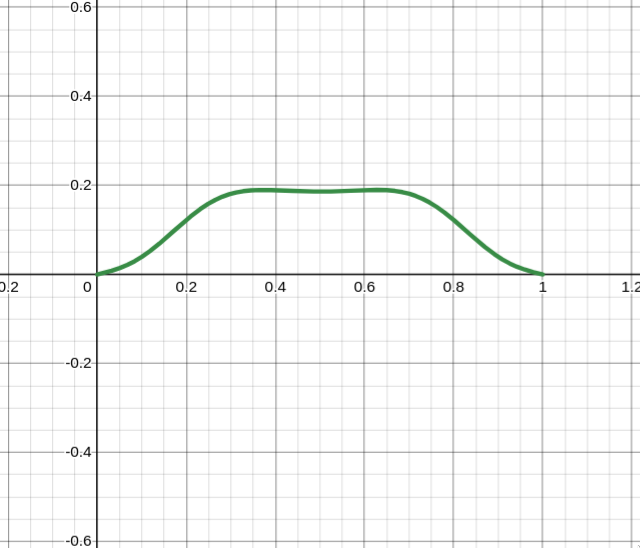
\includegraphics[width=0.9\textwidth]{../phys311/ss/d_n_02.png}
	\caption{$t = \frac{\tau}{3} = \frac{2}{3}$}
	\label{fig:ss-c_n_01-png}
\end{figure}
\begin{figure}[H]
	\centering
	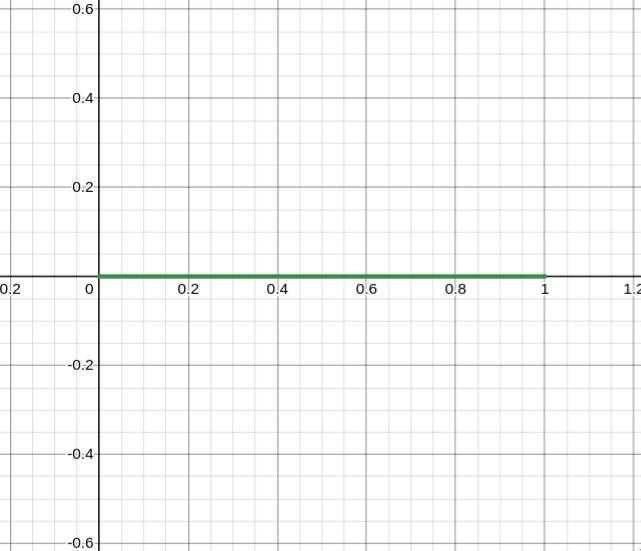
\includegraphics[width=0.9\textwidth]{../phys311/ss/d_n_03.png}
	\caption{$t = \frac{\tau}{2} = 1$}
	\label{fig:ss-c_n_01-png}
\end{figure}
\end{minipage}
\newpage

\begin{minipage}{0.5\textwidth}
\begin{figure}[H]
	\centering
	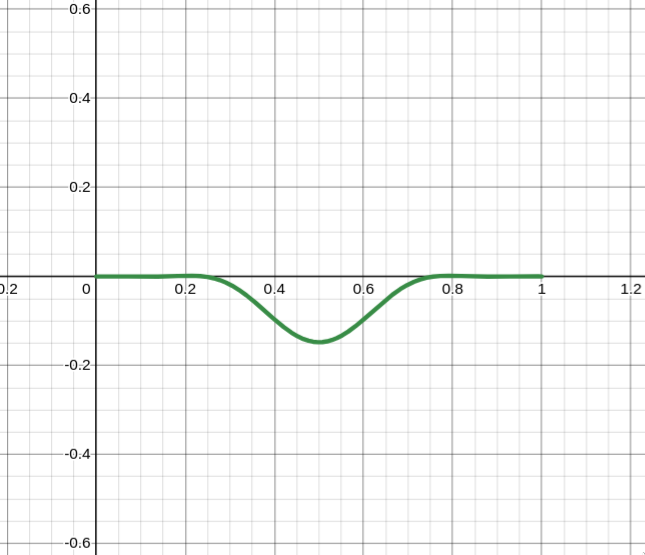
\includegraphics[width=0.9\textwidth]{../phys311/ss/dx1.png}
	\caption{$t = 1.1$}
	\label{fig:ss-c_n_001-png}
\end{figure}
\begin{figure}[H]
	\centering
	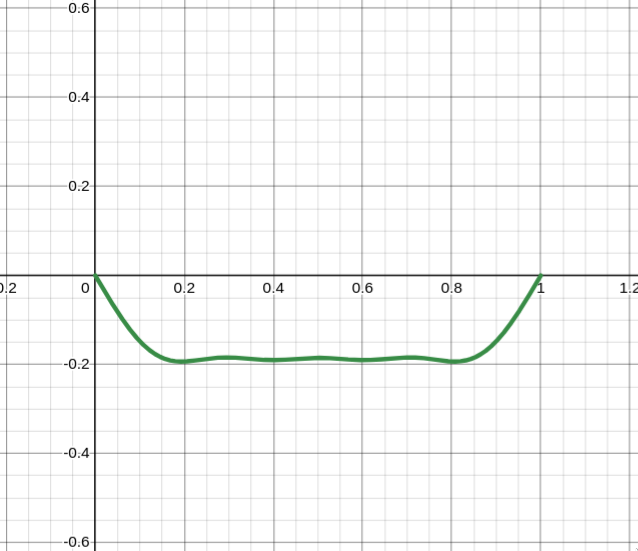
\includegraphics[width=0.9\textwidth]{../phys311/ss/dx2.png}
	\caption{$t =  1.5 $}
	\label{fig:ss-c_n_01-png}
\end{figure}
\end{minipage}
\hfill %
\begin{minipage}{0.5\textwidth}
\begin{figure}[H]
	\centering
	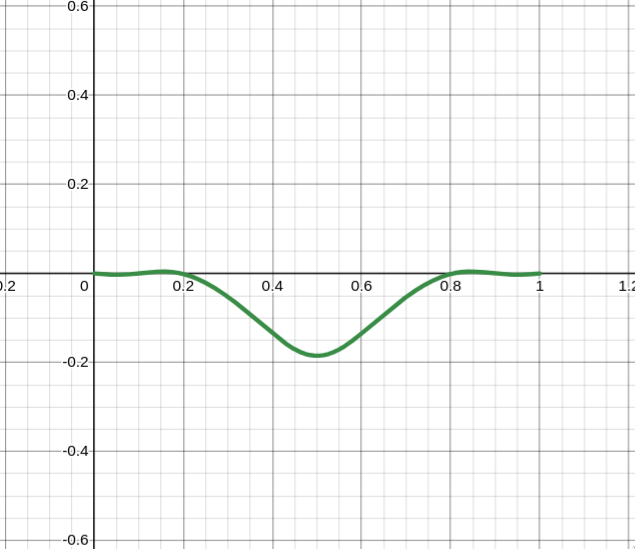
\includegraphics[width=0.9\textwidth]{../phys311/ss/dx3.png}
	\caption{$t = 1.85$}
	\label{fig:ss-c_n_01-png}
\end{figure}
\begin{figure}[H]
	\centering
	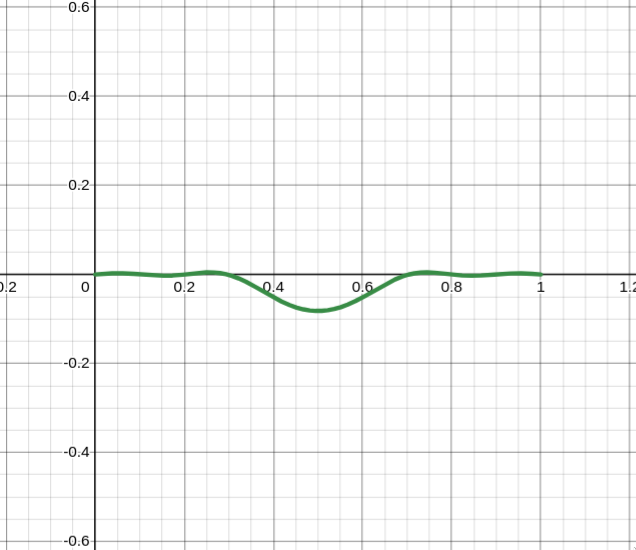
\includegraphics[width=0.9\textwidth]{../phys311/ss/dx4.png}
	\caption{$t = 1.95$}
	\label{fig:ss-c_n_01-png}
\end{figure}
\end{minipage}
\newpage




\section*{Handwritten scratchwork as promised} 
\hrule 
\begin{figure}[H]
	\centering
	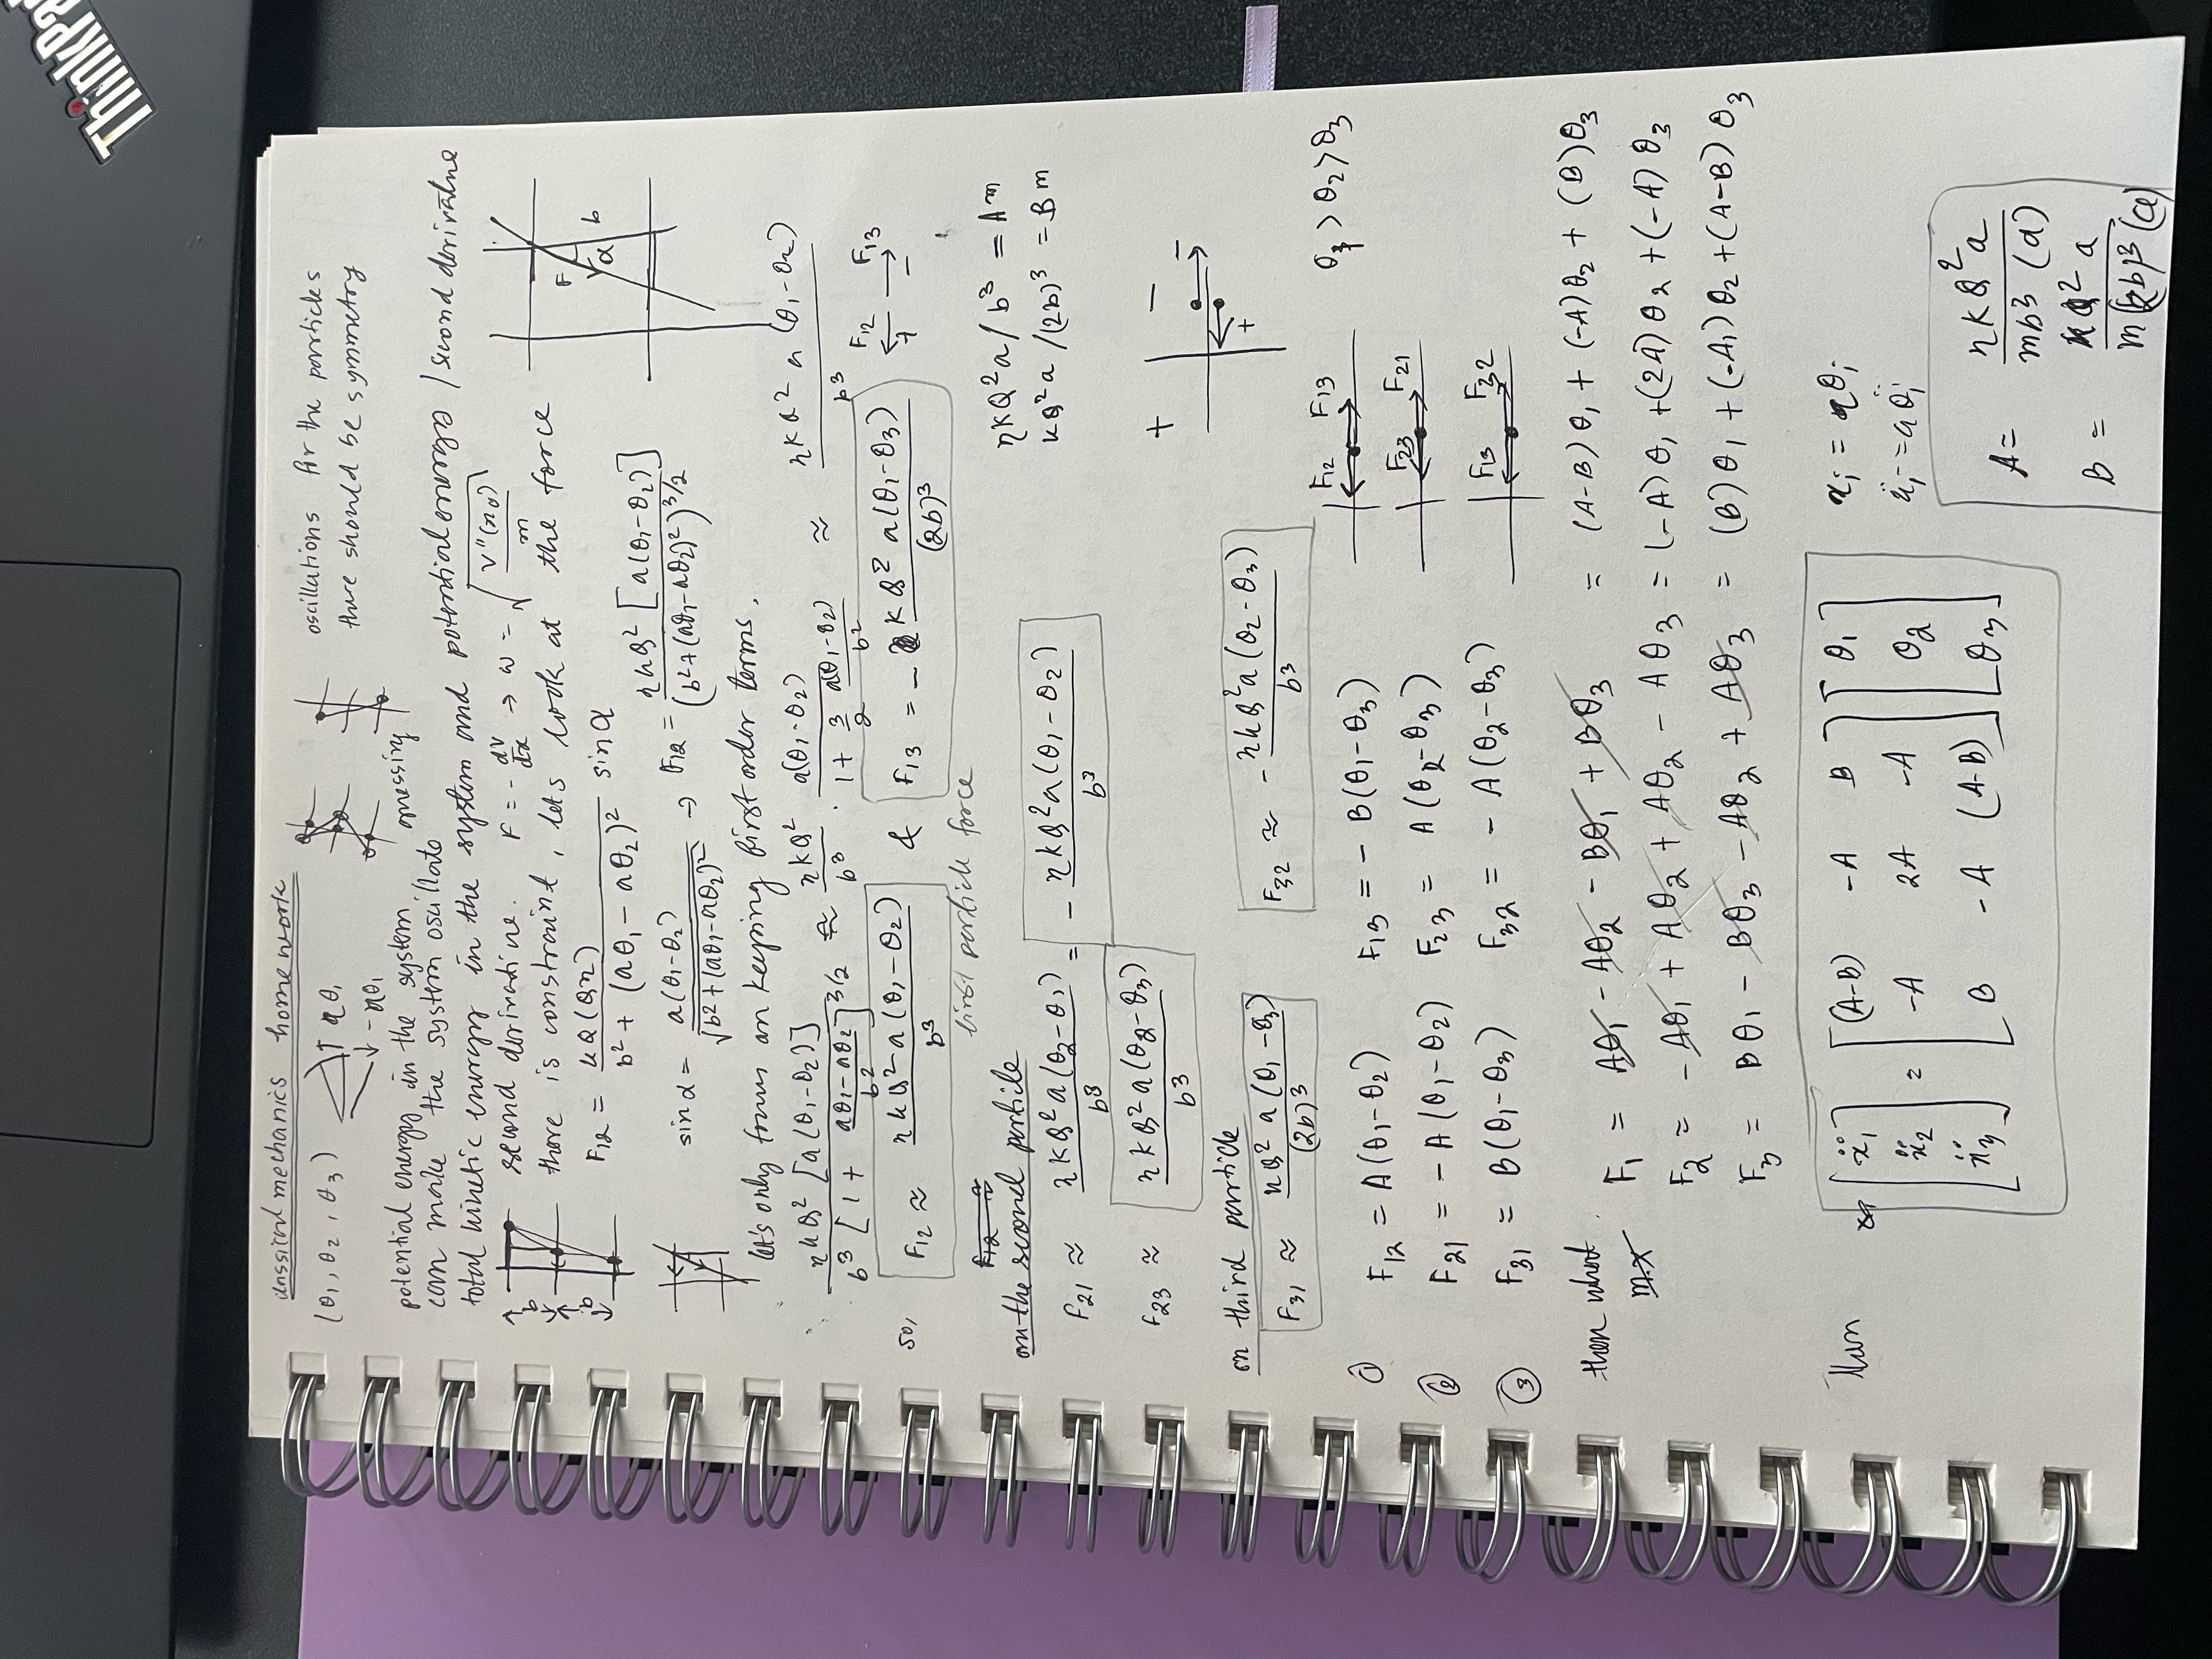
\includegraphics[angle=270, width=0.9\textwidth]{../phys311/ss/11/5.jpeg}
	\caption{../phys311/ss/11/76.jpeg}
	\label{fig:-phys311-ss-11-76-jpeg}
\end{figure}

\begin{figure}[H]
	\centering
	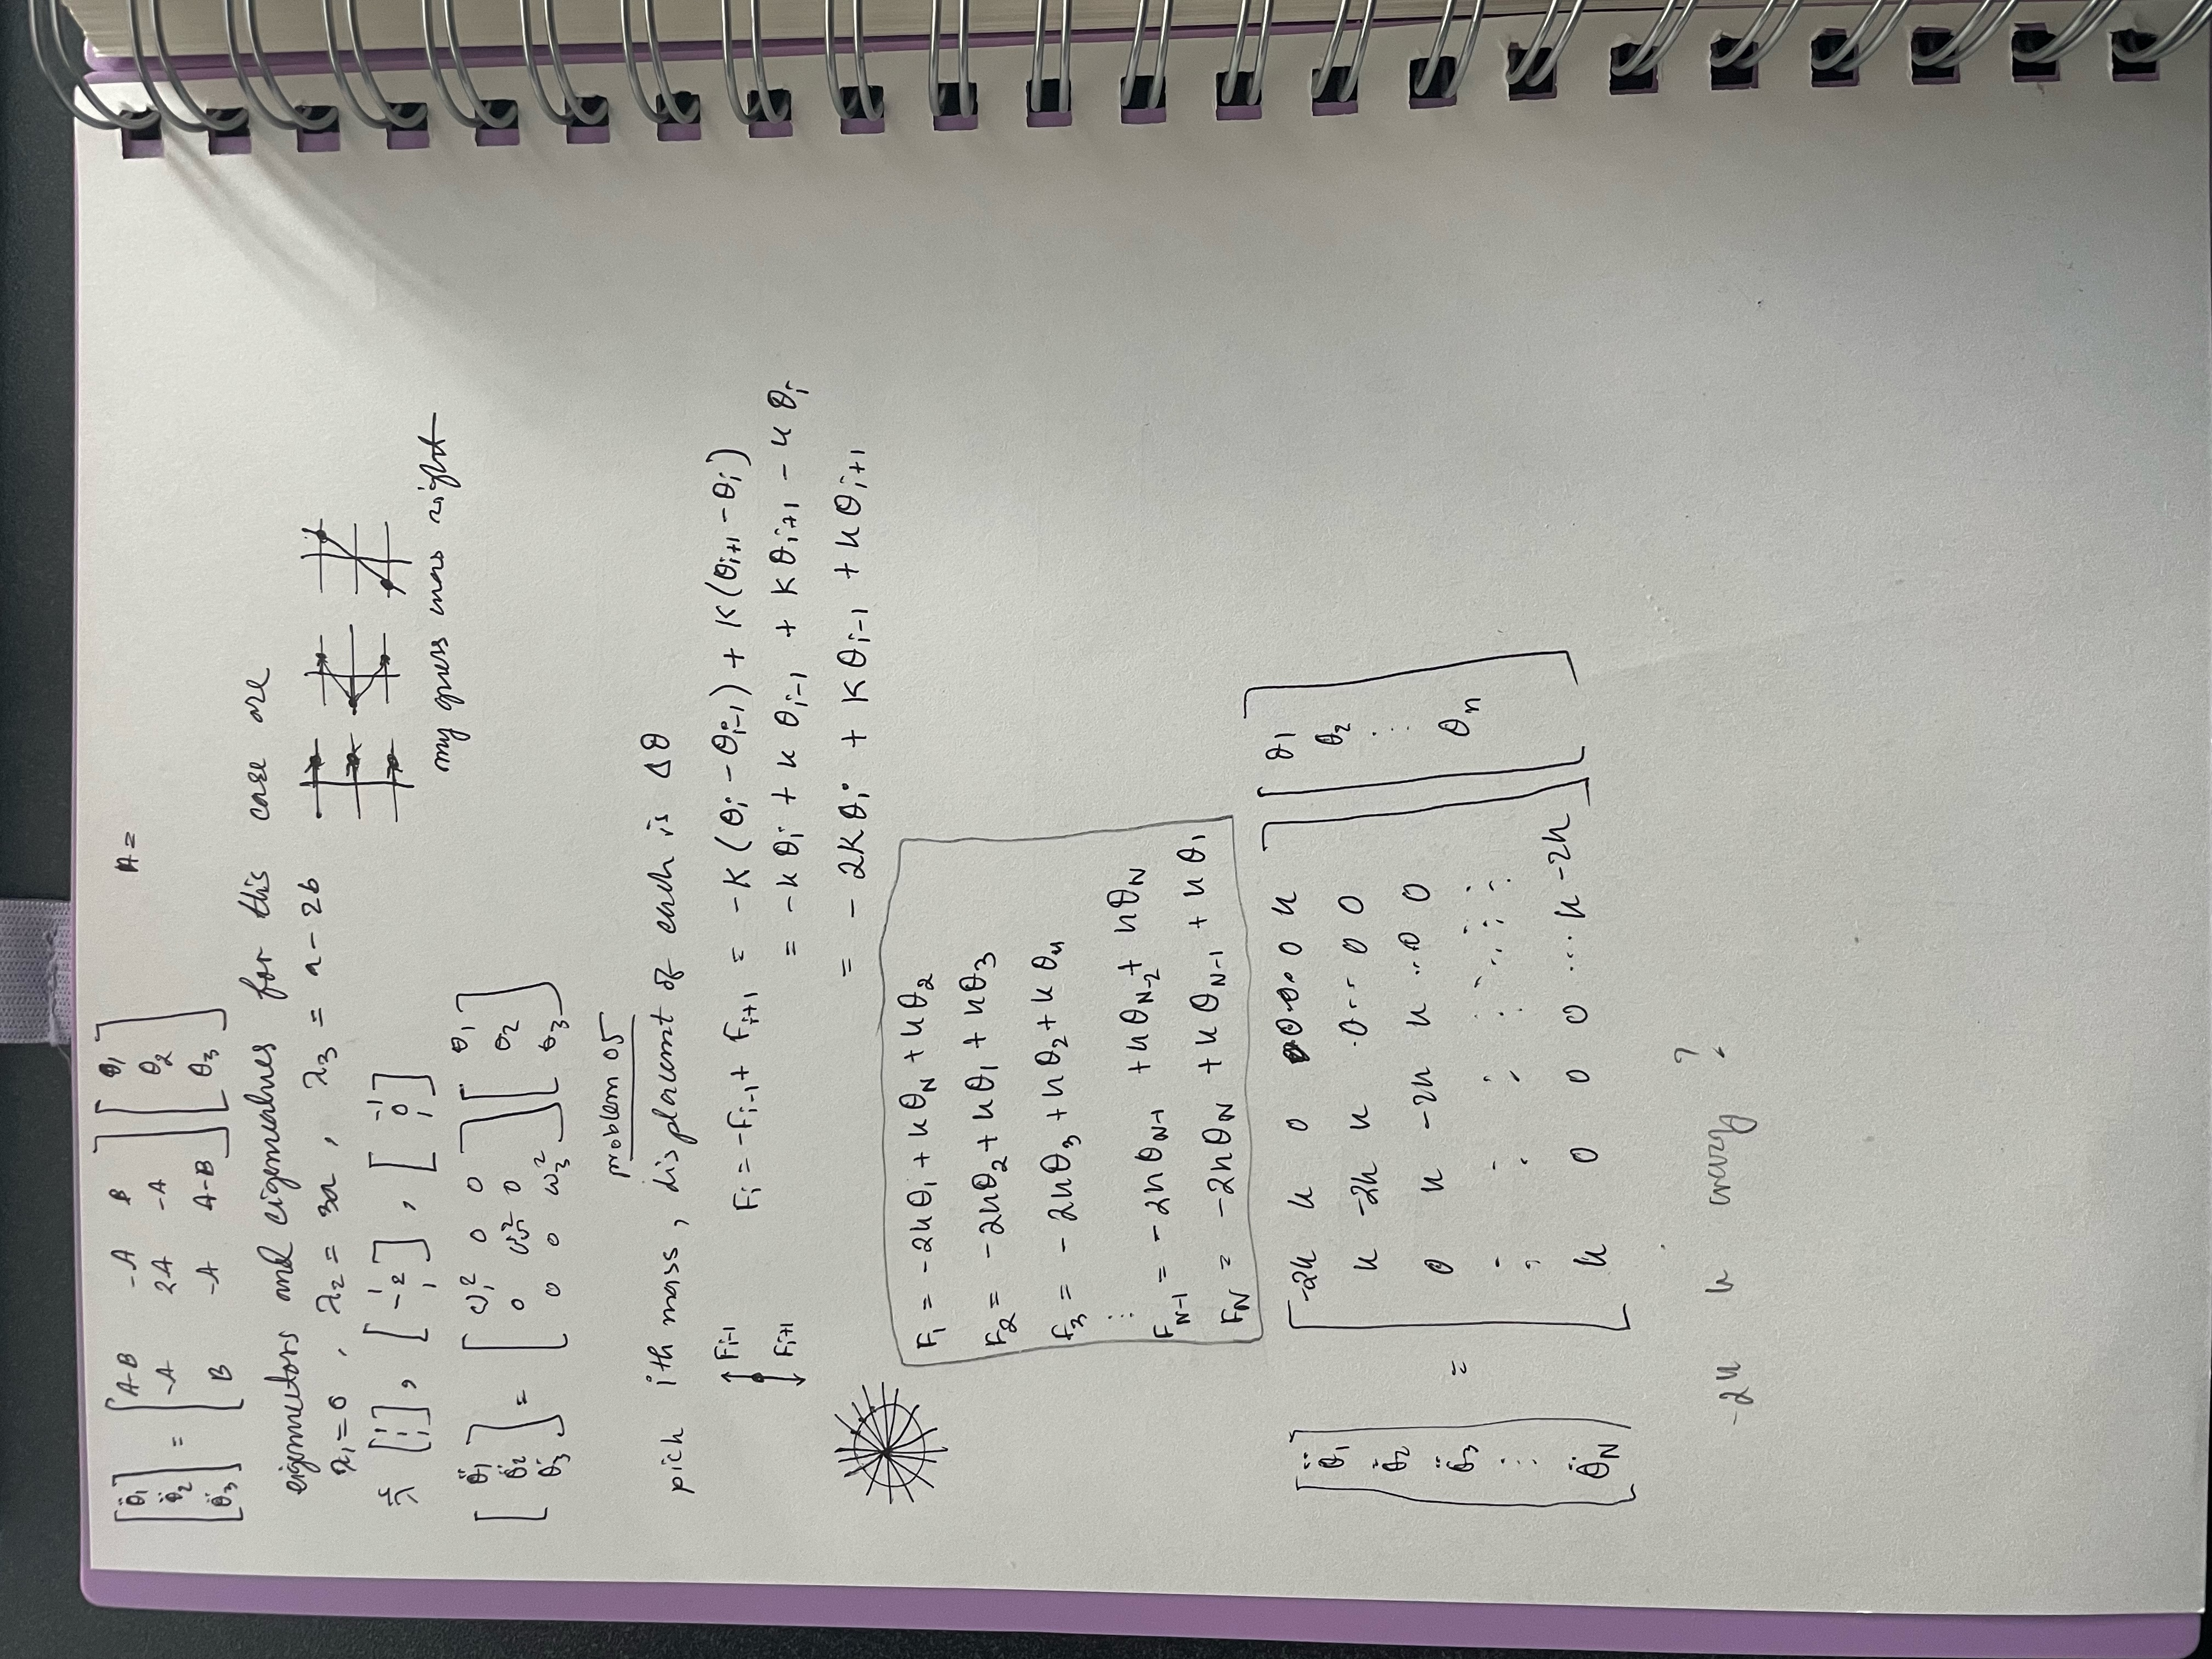
\includegraphics[angle=270, width=0.9\textwidth]{../phys311/ss/11/76.jpeg}
	\caption{../phys311/ss/11/76.jpeg}
	\label{fig:-phys311-ss-11-76-jpeg}
\end{figure}

\end{document}
